\documentclass[a4paper,12pt,titlepage]{report}
\usepackage[utf8]{inputenc}
\usepackage{graphicx} % Required for inserting images
\usepackage[spanish,es-tabla]{babel}
\usepackage[none]{hyphenat}
\usepackage[justification=centering]{caption}
\usepackage{subcaption}
\usepackage{amssymb, amsmath}
\usepackage{gensymb}
\usepackage{fancyhdr}
\usepackage{wrapfig}
\usepackage{hyperref}
\usepackage{longtable}

\setcounter{secnumdepth}{3}


\lhead{Laboratorio de electricidad}
\rhead{Gonzalo Bastos González}

\pagestyle{fancy}

\title{Laboratorio de electricidad}
\author{Gonzalo Bastos González}



\begin{document}

\begin{titlepage}
    \centering
    {\bfseries\LARGE Universidade de Santiago de Compostela \par}
    \vspace{3cm}
    {\scshape\Huge Laboratorio de electricidad \par}
    \vspace{3cm}
    {\scshape\Large Técnicas experimentales I \par}
    \vspace{1cm}
    {\scshape\Large Grado en Física, curso 2022-2023 \par}
    \vfill
    {\Large Gonzalo Bastos Gonzáles \par}
    {\Large GL 1, pareja 6 \par}
    \vspace{3cm}
    \end{titlepage}

\tableofcontents

\footnote{Ajuste por mínimos cuadrados detallado en la parte de mecánica}

\chapter{Bobinas Helmholtz}

\section{Introducción teórica}

El objetivo de esta práctica es medir el campo magnético axial creado por dos bobinas paralelas variando la distancia que las separa. La configuración experimental que vamos a adoptar, conocida como bobinas de Helmholtz, tiene la particularidad de que cuando la distancia que separa a las bobinas es igual a su radio el campo magnético creado por las bobinas en su interior es prácticamente constante, algo que comprobaremos experimentalmente. Esta particularidad hace que las bobinas de Helmholtz sean muy útiles en experimentos en los que se necesita trabajar con campos magnéticos constantes.

\par La expresión del campo magnético creado por las bobinas es la siguiente:

\begin{equation}
    B=\frac{\mu_0 I N}{2 R}\left[\frac{1}{\left(1+\left(\frac{z-a / 2}{R}\right)^2\right)^{3 / 2}}+\frac{1}{\left(1+\left(\frac{z+a / 2}{R}\right)^2\right)^{3 / 2}}\right]
    \label{Campo magnético}
\end{equation}

Las variables de las que depende son:

\begin{itemize}
    \item $\mu_{0} = 4\pi \cdot 10^{-7} \; T\cdot m \cdot A^{-1}$ (Permeabilidad magnética del vacío)
    \item $R= 0,20 \; m$ (Radio de las bobinas)
    \item $a =$ Distancia entre bobinas (m)
    \item $I=$ Intensidad que circula por las bobinas (A)
    \item $N=154$ (Número de espiras)
    \item $z=$ Distancia desde el punto medio del segmento que une los centros de las bobinas, que denominaremos origen de medidas, hasta un punto del eje de las mismas (m)
\end{itemize}


\section{Materiales y metodología}

Los materiales empleados en la práctica son:

\begin{itemize}
    \item Dos bobinas de 20 cm de radio
    \item Fuente de alimentación que proporcionará la intensidad que va a circular por las bobinas
    \item Amperímetro para medir esa intensidad de corriente
    \item Teslámetro con una sonda Hall para medir el campo magnético
    \item Regla y metro rígido para medir las diferentes distancias
\end{itemize}

La disposición empleada se muestra en la siguiente figura salvo una pequeña excepción, nuestra sonda Hall se dispone paralela al eje de las bobinas, por lo que se encuentra situada sobre el eje X de la segunda imagen y de desplazará sobre él para medir los diferentes valores de z.

\begin{figure}[h!]
    \begin{subfigure}{0.6\textwidth}
        \centering
        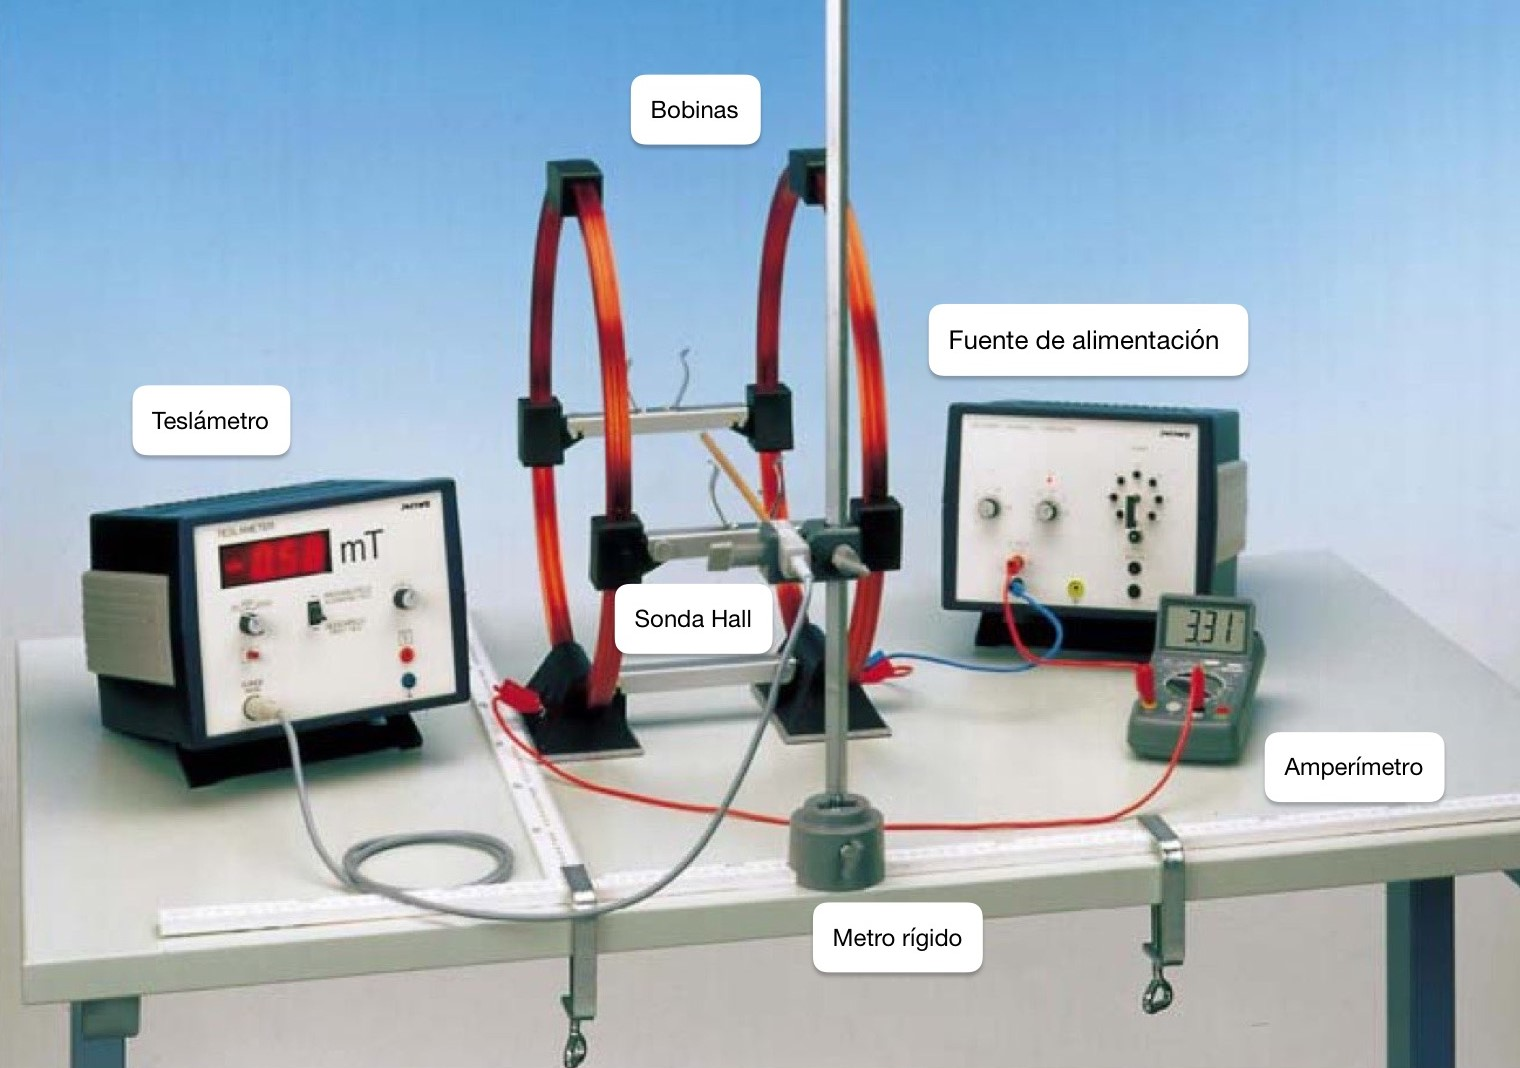
\includegraphics[width=0.95\linewidth]{Images/Bobinas configuración-1.jpg}
    \end{subfigure}
    \begin{subfigure}{0.52\textwidth}
        \centering
        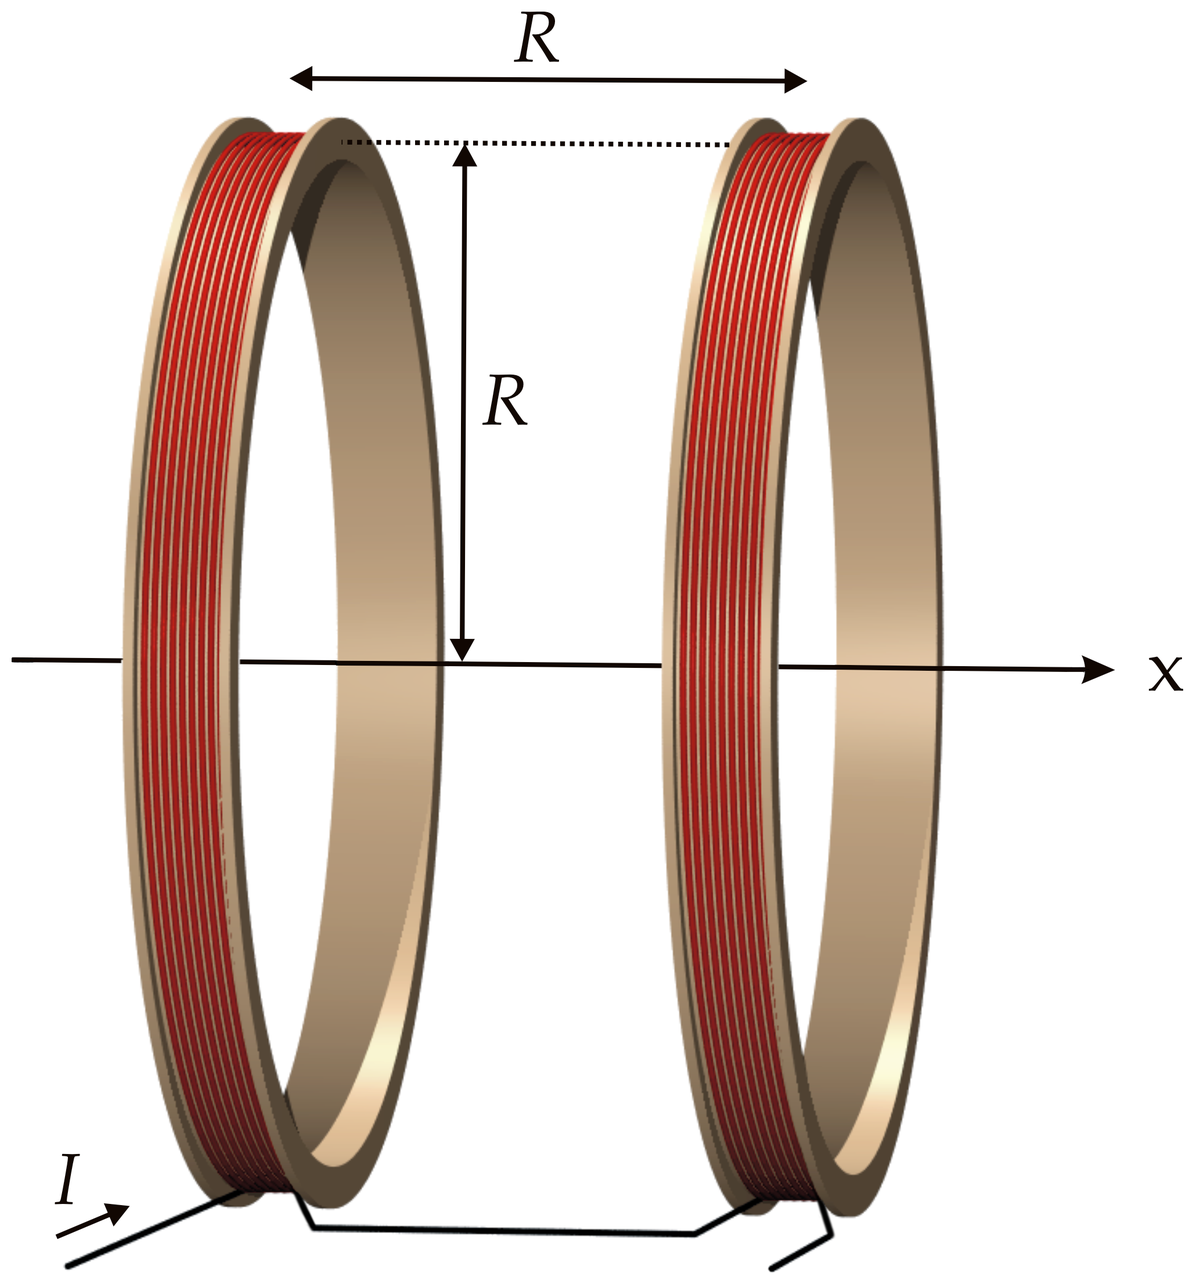
\includegraphics[width=0.75\linewidth]{Images/bobinas esquema.png}
    \end{subfigure}
    \caption{Montaje experimental de las bobinas Helmholtz}
\end{figure}

\par Esta práctica consta de dos partes bien diferenciadas, el estudio del campo magnético axial creado por las bobinas y la determinación de la constante de permeabilidad magnética. La metodología seguida en cada parte se detallará a continuación:

\subsection{Estudio del campo magnético axial}

El objetivo de esta práctica es medir experimentalmente el campo magnético creado por las bobinas a lo largo de su eje, variando las distancias que las separa. Tomaremos medidas en tres situaciones diferentes, variando el valor de $a$, la separación entre bobinas. En primer lugar estudiaremos el campo magnético con $a=R$, luego con $a=2R$ y, por último, con $a=R/2$. Para cada una de estas tres situaciones tomaremos alrededor de 60 valores del valor del campo magnético ($B_{exp}$) frente a diferentes valores de $z$, desplazando la sonda a lo largo del eje, a una intensidad constante de 3 A. Las incertidumbres de los aparatos de medida con los que trabajamos son las siguientes:

\begin{itemize}
    \item La incertidumbre de los valores medidos del campo magnético viene dada por la precisión del teslámetro:
    
    \begin{equation}
        s(B_{exp}) = 0,01\; mT = 10^{-5} \; T
        \label{Inc campo magnético}
    \end{equation}

    \item La incertidumbre de la intensidad viene dada por la precisión de la fuente de alimentación:
    
    \begin{equation}
        s(I) = 0,01 \; A
        \label{Inc intensidad}
    \end{equation}

    \item La incertidumbre de los valores de $z$ la obtendremos de forma indirecta. El método usado para medir los diferentes valores de $z$ fue fijar el cero en un determinado valor de nuestra recta y medir los valores de $z$ calculando el valor absoluto de la resta entre el valor del cero y el valor que medimos. El valor de z se obtiene de la siguiente a partir de la siguiente fórmula:
    
    \begin{equation}
        z = \vert x_0 - x \vert
        \label{Calculo de z}
    \end{equation}

    Donde $x_0$ es el valor del cero y $x$ el valor de separación medido. A partir de esta fórmula obtenemos solo valores de $z$ positivos, no obstante nosotros vamos a definir nuestro propio criterio de signos para diferenciar valores tomados a un lado o el otro del origen de medidas. Los valores de $z$ a la izquierda del origen de medidas serán negativos, mientras que los valores de $z$ a la derecha del origen serán positivos. Las incertidumbre de estos valores las obtendremos a partir de propagación de incertidumbres mediante la siguiente fórmula:

    \begin{equation}
        s(z) = \sqrt{\left (\frac{\partial z}{\partial x_0}\right )^2 s^2(x_0)  + \left (\frac{\partial z}{\partial x} \right )^2 s^2(x)} = \sqrt{s^2(x_0) + s^2(x)}
    \end{equation}

    Las incertidumbres de $x$ y $x_0$ vienen dadas por la precisión de la regla y son iguales, por lo que la incertidumbre de $z$ queda de la siguiente forma:

    \begin{equation}
        s(x) = s(x_0) = 1 \; mm = 10^{-3} \; m \Rightarrow s(z) = \sqrt{2} \cdot s(x) = \sqrt{2} \cdot 10^{-3} \; m
        \label{Inc z}
    \end{equation}
\end{itemize}

Una vez tengamos nuestros puntos con sus respectivas incertidumbres debemos comparar las medidas experimentales con el valor teórico que deberían tener, para ello calcularemos los valores teóricos ($B_T$) del campo a partir de la Ec.\ref{Campo magnético} para cada valor de $z$ con el que trabajamos. De esa forma obtendremos dos conjuntos de datos para el campo magnético, que compararemos para determinar la precisión de nuestras medidas. Una forma de realizar esa comparación es calcular la desviación cuadrática media, a partir de la siguiente ecuación:

\begin{equation}
    s = \frac{1}{N} \sqrt{\sum_{i=1}^{n} (B_{exp} - B_T)^2}
    \label{Desviación cuadrática media}
\end{equation}

Otra forma de comprobar esa correlación entre los datos experimentales y teóricos es de forma gráfica. Es por eso que realizaremos una representación para cada una de las tres situaciones de los puntos experimentales y la curva teórica. Por último, hay que destacar que nuestras curvas van a aparecer incompletas, algo que se va a notar especialmente cuando las representemos gráficamente. Esto se debe a que el carril por donde se mueve la sonda tiene un cierto tope, al encontrarse con las bobinas, y la sonda no puede seguir avanzando para medir más allá de cierto valor de $z$. Una posible solución a este problema sería invertir la polaridad al circuito, pero para la realización de esta práctica se decidió simplemente no tomar los valores a partir de ahí, puesto que para estudiar el comportamiento de la curva, que es simétrica respecto al origen, nos valdría incluso con estudiar solo un lado.

\newpage

\subsection{Determinación de la permeabilidad magnética}

La segunda parte de la práctica consistirá en la determinación de la permeabilidad magnética del vacío ($\mu_0$) relacionando esta constante con el valor del campo magnético que crean en el origen de medidas ($z=0$) diferentes valores de intensidad de corriente. La forma de relacionar estas magnitudes es a partir de la Ec.\ref{Campo magnético}, realizando un ajuste por mínimos cuadrados para ajustar $B$ frente a $I$ y la pendiente de ese ajuste estará directamente relacionada con la constante $\mu_0$. A continuación detallaremos el tratamiento matemático que justifica ese ajuste.

\par Como el valor de $z$ es constante y además es igual a cero la Ec.\ref{Campo magnético} se transforma en:

\begin{equation}
    B=\frac{\mu_0 I N}{2 R}\left[\frac{2}{\left(1+\frac{a^2}{4R^2}\right)^{3 / 2}}\right]
\end{equation}

Para facilitar los cálculos denominaremos $\gamma$ a siguiente factor:

\begin{equation}
    \gamma = \frac{2}{\left(1+\frac{a^2}{4R^2}\right)^{3 / 2}}
    \label{Factor gamma}
\end{equation}

Si nos fijamos en las dependencias del factor $\gamma$ podemos ver que solo depende del valor de $a$, la separación entre las bobinas. No obstante, el valor de $a$ no cambia a lo largo de las medidas que realizamos de $B$ frente a $I$. Por tanto podemos tomar $\gamma$ como una constante, que no resulta ser más que un factor de escala que indica que el valor del campo es inversamente proporcional a la distancia que separa a las bobinas, hablando de forma bastante generalizada pues la dependencia no es lineal.

\par Tratar al factor $\gamma$ como una constante nos facilita mucho la vida a la hora de realizar nuestro ajuste, transformando la ecuación del campo en:

\begin{equation}
    B=\frac{\mu_0 \gamma N}{2 R} I
    \label{Ec campo reducida}
\end{equation}

A partir de esta simplificación de la ecuación del campo ya podemos obervar con claridad que $B$ e $I$ presentan una clara dependencia lineal. Si realizamos nuestro ajuste de métodos cuadrados podemos aproximar nuestros datos a una recta de regresión sin término independiente ($y=bx$) cuya pendiente sería:

\begin{equation}
    b = \frac{\mu_0 \gamma N}{2 R}
\end{equation}

A partir de esta expresión podemos calcular a partir de nuestros datos experimentales la constante de permeabilidad magnética, despejándola de la ecuación anterior:

\begin{equation}
    \mu_0 = \frac{2bR}{\gamma N}
    \label{Permeabilidad magnética}
\end{equation}

La incertidumbre de la constante se obtendrá a partir de propagación de incertidumbres, teniendo en cuenta la incertidumbre del factor $\gamma$, que calcularemos a continuación, y la incertidumbre de la pendiente de la recta de regresión.

\par La incertidumbre de $\gamma$ viene dada por la siguiente expresión:

\begin{equation}
    s(\gamma) = \sqrt{\left (\frac{\partial \gamma}{\partial a}\right )^2 s^2(a)} = \frac{3a}{2R^2 \left (1+ \frac{a^2}{4R^2} \right )^{5/2}} s(a)
\end{equation}

Por tanto, la incertidumbre de permeabilidad magnética $\mu_0$ viene dada por la siguiente expresión:

\begin{equation}
    \begin{gathered}
    s(\mu_0) = \sqrt{\left (\frac{\partial \mu_0 }{\partial b} \right )^2s^2(b) + \left (\frac{\partial \mu_0}{\partial \gamma} \right )^2s^2(\gamma)} = \sqrt{\frac{4R^2}{\gamma^2 N^2} s^2(b) + \frac{4b^2R^2}{\gamma^4 N^2} s^2(\gamma)} \\
    s(\mu_0) = \frac{2R}{\gamma N} \sqrt{s^2(b) + \frac{b^2}{\gamma ^2}s^2(\gamma)}
    \end{gathered}
    \label{Incertidumbre permeabilidad}
\end{equation}

Una vez explicada la metodología experimental de ambas partes de la práctica procederemos a realizar el análisis de los datos medidos.

\newpage

\section{Análisis de datos}

\subsection{Estudio del campo magnético axial}

Una vez detallada la metodología que vamos a seguir vamos a proceder con el análisis de los datos obtenidos en el laboratorio. Trataremos por separado los valores medidos para cada una de las 3 distancias entre las bobinas:

\subsubsection{$\mathbf{a=R}$}

En la siguiente tabla representaremos los valores del campo magnético medidos para cada valor de $z$, así como el valor teórico que le corresponde, calculado a partir de la Ec.\ref{Campo magnético}:

\begin{longtable}[t]{|c|c|c|c|c|c|}
    \hline
    $z \; (cm)$ & $B_{exp} \; mT$ & $B_T \; mT$ & $z \; (cm)$ & $B_{exp} \; mT$ & $B_T \; mT$ \\ \hline
    0      & 1,95 & 2.08 & -24,7 & 0,89 & 0.94 \\ \hline
    -1,1   & 1,94 & 2.08 & -25,4 & 0,85 & 0.89 \\ \hline
    -2,9   & 1,95 & 2.08 & -26   & 0,81 & 0.86 \\ \hline
    -3,4   & 1,95 & 2.08 & -26,6 & 0,77 & 0.82 \\ \hline
    -4,7   & 1,95 & 2.07 & -27,4 & 0,72 & 0.78 \\ \hline
    -5,7   & 1,94 & 2.06 & -28,1 & 0,69 & 0.74 \\ \hline
    -6,4   & 1,94 & 2.05 & -28,8 & 0,66 & 0.70 \\ \hline
    -6,9   & 1,93 & 2.05 & -29,5 & 0,63 & 0.67 \\ \hline
    -7,3   & 1,92 & 2.04 & -30,1 & 0,6  & 0.64 \\ \hline
    -7,4   & 1,91 & 2.04 & -30,7 & 0,58 & 0.61 \\ \hline
    -7,7   & 1,91 & 2.03 & -31,4 & 0,55 & 0.58 \\ \hline
    -8,4   & 1,9  & 2.02 & -32,2 & 0,52 & 0.55 \\ \hline
    -8,9   & 1,88 & 2.00 & -32,9 & 0,49 & 0.52 \\ \hline
    -9,4   & 1,87 & 1.99 & -34,4 & 0,45 & 0.47 \\ \hline
    -10    & 1,86 & 1.96 & -35   & 0,43 & 0.45 \\ \hline
    -10,4  & 1,83 & 1.95 & -35,5 & 0,42 & 0.44 \\ \hline
    -10,9  & 1,81 & 1.93 & -36,2 & 0,4  & 0.42 \\ \hline
    -11,5  & 1,77 & 1.90 & -37   & 0,38 & 0.39 \\ \hline
    -12,2  & 1,76 & 1.86 & -37,6 & 0,37 & 0.38 \\ \hline
    -12,8  & 1,71 & 1.83 & -38,4 & 0,35 & 0.36 \\ \hline
    -13,4  & 1,69 & 1.79 & 0,6   & 1,94 & 2.08 \\ \hline
    -14    & 1,64 & 1.75 & 1,4   & 1,94 & 2.08 \\ \hline
    -14,5  & 1,6  & 1.71 & 2,1   & 1,94 & 2.08 \\ \hline
    -14,94 & 1,57 & 1.68 & 2,9   & 1,94 & 2.08 \\ \hline
    -15,4  & 1,55 & 1.65 & 3,8   & 1,94 & 2.07 \\ \hline
    -15,9  & 1,51 & 1.61 & 4,6   & 1,93 & 2.07 \\ \hline
    -16,5  & 1,47 & 1.57 & 5,4   & 1,93 & 2.07 \\ \hline
    -17    & 1,43 & 1.53 & 6,1   & 1,94 & 2.06 \\ \hline
    -17,6  & 1,39 & 1.48 & 6,9   & 1,92 & 2.05 \\ \hline
    -18,4  & 1,32 & 1.41 & 7,8   & 1,91 & 2.03 \\ \hline
    -19    & 1,27 & 1.37 & 8,5   & 1,9  & 2.01 \\ \hline
    -19,5  & 1,23 & 1.33 & 9,4   & 1,86 & 1.99 \\ \hline
    -20    & 1,2  & 1.29 & 10,2  & 1,84 & 1.96 \\ \hline
    -20,5  & 1,17 & 1.25 & 11,3  & 1,8  & 1.91 \\ \hline
    -20,9  & 1,13 & 1.22 & 12,1  & 1,75 & 1.87 \\ \hline
    -21,5  & 1,1  & 1.17 & 12,7  & 1,72 & 1.83 \\ \hline
    -22,4  & 1,02 & 1.10 & 13,2  & 1,7  & 1.80 \\ \hline
    -23    & 1    & 1.06 & 13,6  & 1,67 & 1.78 \\ \hline
    -23,5  & 0,96 & 1.02 & 14,2  & 1,64 & 1.74 \\ \hline
    -24,1  & 0,92 & 0.98 & 14,8  & 1,6  & 1.69 \\ \hline
    \caption{Valores experimentales y teóricos del campo magnético para $a=R$}
    \label{Datos aR}
\end{longtable}


A partir de estos datos debemos calcular la desviación cuadrática media entre los valores experimentales y teóricos del campo para determinar la exactitud de nuestras medidas. Para ello emplearemos la Ec.\ref{Desviación cuadrática media} y el resultado obtenido fue el siguiente:

\begin{equation}
    s = \frac{1}{N} \sqrt{\sum_{i=1}^{n} (B_{exp} - B_T)^2} = 0.087 \; mT
\end{equation}

Para tener una idea más gráfica de la correlación de las medidas en la siguiente figura representaremos el valor del campo magnético en función de $z$:

\newpage

\begin{figure}[h!]
    \centering
    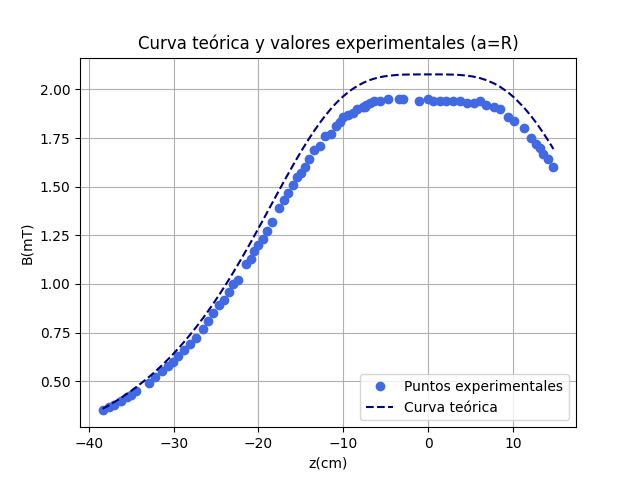
\includegraphics[width=0.85\linewidth]{Images/CurvaB1.png}
    \caption{Representación gráfica de los datos para $a=R$}
\end{figure}

Como hemos mencionado anteriormente, los valores de $z$ negativos son aquellos que se encuentran a la izquierda de las bobinas mientras que los positivos son aquellas medidas realizadas a la deerecha de las bobinas. En la gráfica se puede apreciar claramente que en los puntos interiores a las dos bobinas ($-10<z<10$) los valores del campo teórico y experimental difieren de forma notable. Esto se debe, como explicaremos al final de la sección, a un problema con la fuente de alimentación.

\subsubsection{$\mathbf{a=R/2}$}

Para el valor $a=R/2$ el procedimiento será el mismo, representaremos los valores del campo magnético teóricos y experimentales en una tabla, calcularemos su desviación cuadrática media y realizaremos una representación gráfica de los datos. En la siguiente tabla veremos los datos del campo magnético para diferentes valores de $z$:

\newpage

\begin{longtable}[t]{|c|c|c|c|c|c|}
    \hline
    $z \; (cm)$ & $B_{exp} \; mT$ & $B_T \; mT$ & $z \; (cm)$ & $B_{exp} \; mT$ & $B_T \; mT$ \\ \hline
    0.00     & 2.41 & 2.65 & -21.9 & 0.89 & 0.96 \\ \hline
    -1.2  & 2.40 & 2.64 & -23.6 & 0.77 & 0.84 \\ \hline
    -0.7  & 2.41 & 2.65 & -24.7 & 0.73 & 0.78 \\ \hline
    -2.4  & 2.38 & 2.61 & -26.9 & 0.62 & 0.66 \\ \hline
    -1.5  & 2.39 & 2.64 & -28.0 & 0.58 & 0.61 \\ \hline
    -2.4  & 2.37 & 2.61 & -29.2 & 0.54 & 0.56 \\ \hline
    -3.4  & 2.34 & 2.58 & -30.8 & 0.48 & 0.5  \\ \hline
    -4.1  & 2.32 & 2.54 & -32.5 & 0.43 & 0.45 \\ \hline
    -4.6  & 2.30 & 2.51 & -34.0 & 0.40 & 0.4  \\ \hline
    -5.3  & 2.25 & 2.47 & -35.2 & 0.37 & 0.37 \\ \hline
    -5.8  & 2.22 & 2.44 & -36.5 & 0.33 & 0.34 \\ \hline
    -6.3  & 2.17 & 2.4  & 1.3   & 2.41 & 2.64 \\ \hline
    -7.0  & 2.15 & 2.35 & 1.8   & 2.40 & 2.63 \\ \hline
    -8.2  & 2.06 & 2.24 & 2.5   & 2.39 & 2.61 \\ \hline
    -8.8  & 1.98 & 2.19 & 3.2   & 2.36 & 2.58 \\ \hline
    -9.5  & 1.94 & 2.12 & 4.0   & 2.32 & 2.55 \\ \hline
    -10.2 & 1.87 & 2.05 & 4.8   & 2.27 & 2.5  \\ \hline
    -11.0 & 1.82 & 1.97 & 5.5   & 2.24 & 2.46 \\ \hline
    -11.4 & 1.76 & 1.93 & 5.2   & 2.21 & 2.48 \\ \hline
    -12.0 & 1.71 & 1.86 & 6.9   & 2.14 & 2.35 \\ \hline
    -12.6 & 1.66 & 1.8  & 7.6   & 2.08 & 2.29 \\ \hline
    -13.1 & 1.60 & 1.75 & 8.3   & 2.03 & 2.23 \\ \hline
    -13.5 & 1.54 & 1.71 & 9.2   & 1.93 & 2.15 \\ \hline
    -14.2 & 1.48 & 1.63 & 10.0  & 1.88 & 2.07 \\ \hline
    -14.7 & 1.44 & 1.58 & 11.5  & 1.74 & 1.91 \\ \hline
    -15.5 & 1.37 & 1.5  & 12.7  & 1.62 & 1.79 \\ \hline
    -16.0 & 1.32 & 1.45 & 13.4  & 1.53 & 1.72 \\ \hline
    -16.9 & 1.25 & 1.37 & 14.5  & 1.45 & 1.6  \\ \hline
    -17.8 & 1.18 & 1.28 & 16.0  & 1.33 & 1.45 \\ \hline
    -19.3 & 1.07 & 1.15 & 17.5  & 1.21 & 1.31 \\ \hline
    -20.5 & 0.98 & 1.06 &       &      &      \\ \hline
    \caption{Valores teóricos y experimentales para $a=R/2$}
\end{longtable}

\newpage

A partir de estos datos debemos calcular la desviación cuadrática media entre los valores experimentales y teóricos del campo para determinar la exactitud de nuestras medidas. Para ello emplearemos la Ec.\ref{Desviación cuadrática media}, el resultado obtenido fue el siguiente:

\begin{equation}
    s = \frac{1}{N} \sqrt{\sum_{i=1}^{n} (B_{exp} - B_T)^2} = 0.091 \; mT
\end{equation}

En la siguiente figura podemos ver una representación gráfica de los valores experimentales y teóricos del campo magnético frente a $z$:

\begin{figure}[h!]
    \centering
    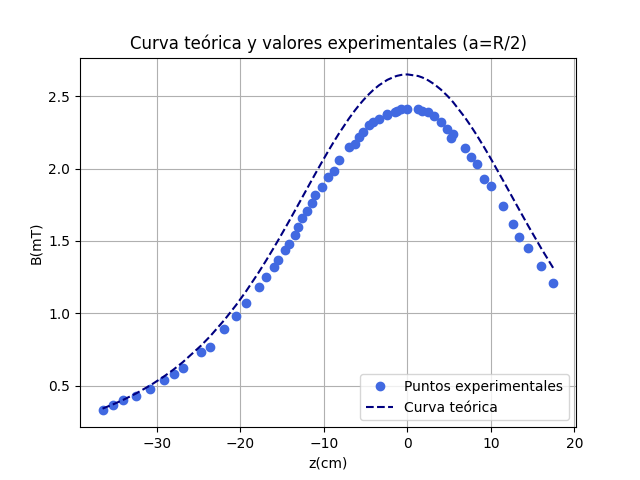
\includegraphics[width=0.85\linewidth]{Images/CurvaB2.png}
    \caption{Representación gráfica de los datos para $a=R/2$}
\end{figure}

Como en el apartado anterior, el valor de la curva teórica es notablemente mayor que el medido experimentalmente para valores de $z$ próximos al origen de coordenadas. Esto se debe, como explicaremos más detalladamente al final de la sección, a un problema con la fuente de alimentación, que no suministraba la suficiente corriente.

\subsubsection{$\mathbf{a=2R}$}

El procedimiento seguido será el mismo que en los apartados anteriores, representaremos en una tabla los valores teóricos y experimentales para diferentes valores de $z$, calcularemos la desviación cuadrática media entre los valores experimentales y teóricos y realizaremos una representación gráfica de los datos. En la siguiente tabla podemos ver los valores del campo magnético experimentales y teóricos en función de $z$:


\begin{longtable}[ht]{|c|c|c|c|c|c|}
    \hline
    $z \; (cm)$ & $B_{exp} \; (mT)$ & $B_T \; (mT)$ & $z \; (cm)$ & $B_{exp} \; (mT)$ & $B_T \; (mT)$ \\ \hline
    0     & 0.95 & 1.03 & -22.2 & 1.47 & 1.54 \\ \hline
    -0.9  & 0.95 & 1.03 & -22.8 & 1.46 & 1.52 \\ \hline
    -1.8  & 0.94 & 1.04 & -23.5 & 1.42 & 1.49 \\ \hline
    -3.   & 0.95 & 1.05 & -24.  & 1.40 & 1.47 \\ \hline
    -3.8  & 0.97 & 1.07 & -24.7 & 1.37 & 1.44 \\ \hline
    -4.5  & 1.00 & 1.08 & -25.5 & 1.34 & 1.4  \\ \hline
    -5.4  & 1.01 & 1.11 & -26.5 & 1.29 & 1.34 \\ \hline
    -6.   & 1.02 & 1.13 & -27.  & 1.26 & 1.31 \\ \hline
    -6.5  & 1.03 & 1.14 & -27.8 & 1.22 & 1.26 \\ \hline
    -7.2  & 1.06 & 1.17 & -28.5 & 1.17 & 1.21 \\ \hline
    -8.   & 1.08 & 1.2  & -29.5 & 1.11 & 1.15 \\ \hline
    -8.5  & 1.11 & 1.22 & -30.9 & 1.03 & 1.05 \\ \hline
    -9.   & 1.12 & 1.24 & -32.  & 1.00 & 0.98 \\ \hline
    -9.4  & 1.13 & 1.26 & -32.1 & 0.96 & 0.98 \\ \hline
    -10.  & 1.15 & 1.29 & -33.3 & 0.89 & 0.9  \\ \hline
    -10.6 & 1.19 & 1.31 & -34.5 & 0.82 & 0.83 \\ \hline
    -11.4 & 1.21 & 1.35 & -35.2 & 0.78 & 0.79 \\ \hline
    -11.9 & 1.23 & 1.37 & -36.  & 0.74 & 0.75 \\ \hline
    -12.4 & 1.26 & 1.4  & -36.8 & 0.70 & 0.7  \\ \hline
    -13.3 & 1.30 & 1.44 & -37.6 & 0.66 & 0.67 \\ \hline
    -14.1 & 1.34 & 1.47 & 0.5   & 0.95 & 1.03 \\ \hline
    -15.  & 1.37 & 1.5  & 1.    & 0.96 & 1.03 \\ \hline
    -15.6 & 1.39 & 1.52 & 1.5   & 0.96 & 1.03 \\ \hline
    -16.2 & 1.41 & 1.54 & 2.    & 0.97 & 1.04 \\ \hline
    -16.8 & 1.43 & 1.56 & 2.5   & 0.99 & 1.04 \\ \hline
    -17.5 & 1.45 & 1.57 & 3.    & 1.00 & 1.05 \\ \hline
    -18.2 & 1.46 & 1.58 & 3.5   & 1.01 & 1.06 \\ \hline
    -19.  & 1.48 & 1.58 & 4.    & 1.02 & 1.07 \\ \hline
    -19.8 & 1.48 & 1.58 & 4.5   & 1.03 & 1.08 \\ \hline
    -20.5 & 1.48 & 1.58 & 5     & 1.04 & 1.1  \\ \hline
    -21.5 & 1.47 & 1.56 &       &      &      \\ \hline
    \caption{Valores experimentales y teóricos del campo magnético para $a=2R$}
    \label{Datos a2R}
\end{longtable}



A partir de estos datos debemos calcular la desviación cuadrática media entre los valores experimentales y teóricos del campo para determinar la exactitud de nuestras medidas. Para ello emplearemos la Ec.\ref{Desviación cuadrática media}, el resultado obtenido fue el siguiente:

\begin{equation}
    s = \frac{1}{N} \sqrt{\sum_{i=1}^{n} (B_{exp} - B_T)^2} = 0.059 \; mT
\end{equation}

En la siguiente figura podemos ver representados gráficamente los valores experimentales y la curva teórica del campo magnético en función de $z$:

\begin{figure}[h!]
    \centering
    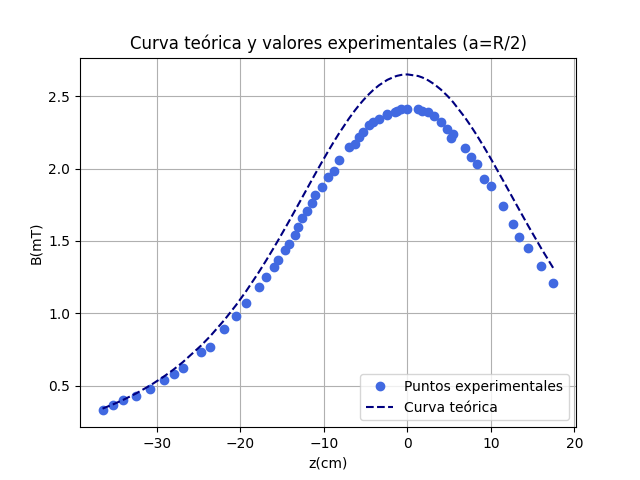
\includegraphics[width=0.85\linewidth]{Images/CurvaB2.png}
    \caption{Representación gráfica de los datos para $a=2R$}
\end{figure}

En la figura se puede observar claramente una discordancia notable entre la curva teórica y los valores experimentales, estando estos notablemente por debajo de lo esperado, especialmente para el intervalo $(-10<z<10)$. Este fenómeno se repitió en las tres medidas y se puede ver claramente en las tres gráficas que los valores experimentales están por debajo de lo esperado en este intervalo. El problema reside en la fuente de alimentación, que aunque estaba fijada en 3 A no suministraba tal intensidad de corriente, solía quedarse en unos 2,8 A. Este problema se nota especialmente en las zonas donde el campo es mayor y por tanto esta discordancia es más perceptible, coincidiendo en el intervalo ($-10<z<10$), que coincide con el interior y las proximidades de las bobinas. Para verificar que efectivamente el problema estaba en el problema con la intensidad de corriente hemos calculado una nueva curva teórica para cada una de las 3 situaciones con una intensidad de corriente de 2,8 A, en vez de los 3 a los que la máquina sospechamos que no llegaba. Gráficamente el resultado es el siguiente:

\begin{figure}[h!]
    \centering
    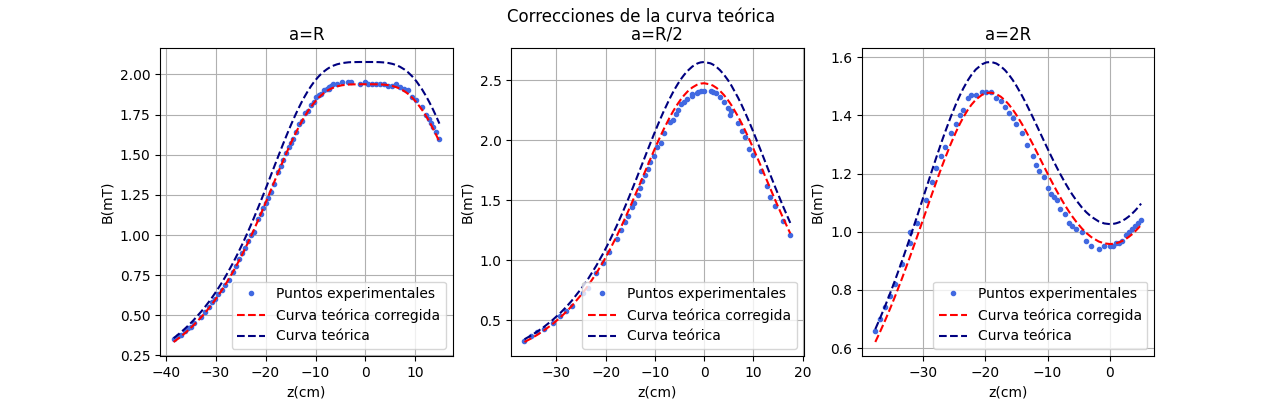
\includegraphics[width=1.20\linewidth]{Images/CurvasCorregidas.png}
    \caption{Curvas corregidas}
    \label{Curvas corregidas}
\end{figure}

Para comprobar matemáticamente nuestra hipótesis vamos a partir de que la intensidad en la Ec.\ref{Campo magnético} es un factor multiplicativo, por lo que el cociente $\frac{B_{T}}{B_{exp}}$ se debería mantener más o menos constante para todos los valores de $z$. Para comprobar esto vamos a calcular la media de estos cocientes y su desviación típica, que debería ser casi nula, según la siguiente expresión:

\begin{equation}
    \begin{gathered}
    \frac{B_{T}}{B_{exp}} = k \Rightarrow \overline{k} = \sum_i^{N} \frac{k_i}{N} \\
    s(k) = \sqrt{\frac{\sum_i^N (x_i-\overline{x})^2}{N-1}}
    \end{gathered}
\end{equation}

Si aplicamos estas fórmulas a los tres valores de $a$ obtenemos cocientes muy próximos a 1 y con desviaciones típicas muy pequeñas. Para $a=R$ la desviación típica es de $0.01$, para $a=R/2$ es de $0.02$ y para $a=2R$ es de $0.03$, que no superan el 3\% del valor de k, que se encuentra entre $1$ y $1,1$ en ambos casos. Por tanto, podemos concluir que, como la desviación típica es muy pequeña en todos los casos y es despreciable, el cociente $k$ es constante. Que este cociente sea constante reafirma nuestra afirmación de que la caída de intensidad de la fuente de alimentación provoca que los valores experimentales medidos estén por debajo de lo previsto.

\newpage

\subsection{Determinación de la permeabilidad magnética}

Como explicamos en la metodología, vamos a calcular la constante de permeabilidad magnética $\mu_0$ a partir de un ajuste por mínimos cuadrado de $B$ frente a $I$, que siguen la relación que se muestra en la Ec.\ref{Ec campo reducida}. Para ello tomamos 15 valores del campo magnético en el origen de coordenadas a diferentes valores de intensidades que representaremos en la siguiente tabla:

\begin{table}[h]
    \centering
    \begin{tabular}{|c|c|}
    \hline
    I (A) & B (mT) \\ \hline
    0,06  & 0,06   \\ \hline
    0,27  & 0,20    \\ \hline
    0,50   & 0,35   \\ \hline
    0,73  & 0,51   \\ \hline
    0,88  & 0,61   \\ \hline
    1,03  & 0,71   \\ \hline
    1,23  & 0,85   \\ \hline
    1,45  & 0,99   \\ \hline
    1,65  & 1,12   \\ \hline
    1,86  & 1,26   \\ \hline
    2,06  & 1,40    \\ \hline
    2,23  & 1,50   \\ \hline
    2,39  & 1,60    \\ \hline
    2,62  & 1,76   \\ \hline
    2,81  & 1,90    \\ \hline
    \end{tabular}
    \caption{Valores experimentales del campo magnético en función de la intensidad}
    \label{tab:my-table}
\end{table}

A partir de estos datos vamos a realizar un ajuste por mínimos cuadrados para ajustar los datos a una recta del tipo $(B=bI)$. Empleamos un ajuste simple sin término independiente porque a intensidad cero no hay campo magnético, este existe por la presencia de la corriente eléctrica circulando por la espira. Los valores obtenidos fueron los siguientes:

\begin{equation}
    \begin{gathered}
        b = 0.0006768 \; T\cdot A^{-1}\\
        s(b) = s(b) = 2.0 \cdot 10^{-6} \; T\cdot A^{-1} \\
        r = 0.99993 \\
        s = 1.3 \cdot 10^{-5}
    \end{gathered}
\end{equation}

En la siguiente figura podemos ver gráficamente el resultado del ajuste por mínimos cuadrados:

\begin{figure}
    \centering
    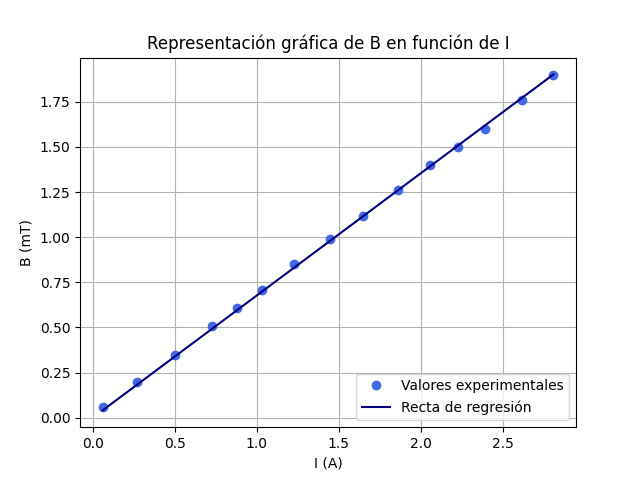
\includegraphics[width=0.85\linewidth]{Images/RegresionPermeabilidad.png}
    \caption{Valores experimentales y regresión de B frente a I}
\end{figure}

A partir de este resultado podemos calcular el valor de la permeabilidad con su incertidumbre aplicando la Ec.\ref{Permeabilidad magnética}, sustituyendo $a=R$ y la Ec.\ref{Incertidumbre permeabilidad}:

\begin{equation}
    \begin{gathered}
        \mu_0 = 1.2284 \cdot 10^{-6}\; T \cdot m \cdot A^{-1} \\
        s(\mu_0) = 3.7 \cdot 10^{-9}\; T \cdot m \cdot A^{-1}
    \end{gathered}
\end{equation}

Para el cálculo de la incertidumbre de $\mu_0$ empleamos la Ec.\ref{Incertidumbre permeabilidad}, como indicamos anteriormente, no obstante debemos notar que la única incertidumbre que participa es $s(b)$, ya que tomamos $\gamma$ como una constante con incertidumbre 0. La justificación matemática de esto es que el valor de $a=R$, a diferencia de los otros dos con los que trabajamos, no fue medido experimentalmente sino que venía determinado por las barras fijas que unían a las bobinas y que tenían una longitud igual a su radio. Es por esto que se decidió tomar este valor como constante y no dotarlo de incertidumbre, pues realmente no es ninguna medida, por lo que la incertidumbre de $\gamma$, que depende de la de $a$, es 0. Por tanto, la incertidumbre de $\mu_0$ viene dada por la siguiente expresión y tiene el valor mencionado anteriormente:

\begin{equation}
    s(\mu_0) = \frac{2R}{\gamma N} s(b)
\end{equation}

\newpage

El valor real de la permeabilidad magnética depende del medio en el que nos encontremos, en el vacío tiene un valor de $\mu_0=4\pi\cdot 10^{-7} \; T \cdot m \cdot A^{-1}$, que es prácticamente el mismo valor que tiene en el aire, por lo que tomaremos ese valor como referencia. Si operamos el valor teórico obtenemos un resultado para la permeabilidad magnética de $1.2566 \cdot 10^{-6}\; T \cdot m \cdot A^{-1}$, que aunque no se encuentra en el rango de incertidumbre se encuentra muy próximo al valor determinado experimentalmente.

\newpage

\section{Conclusión}

La primera parte de la práctica se centró en el estudio del campo magnético axial creado por las dos bobinas. Los resultados experimentales se acercan en gran medida a los valores teóricos, especialmente si tenemos en cuenta la caída de intensidad de la fuente de alimentación. Como podemos ver en la Fig.\ref{Curvas corregidas}, una vez realizamos la corrección de las curvas a una intensidad de $2,8 \;A$ los resultados experimentales se ajustan enormemente a la curva teórica. En la siguiente figura podemos ver los datos de los tres valores de $a$ con los que trabajamos:

\begin{figure}[h!]
    \centering
    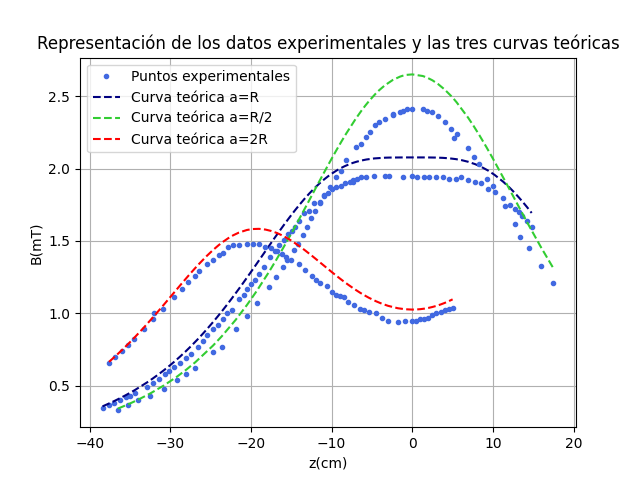
\includegraphics[width=0.95\linewidth]{Images/Tres curvas.png}
    \caption{Gráfica conjunta de las medidas experimentales y las curvas teóricas}
\end{figure}


La segunda parte de la práctica se centró en determinar la constante de permeabilidad magnética. Los resultados también se acercan en gran medida a lo esperado, algo que ya podíamos preveer por el buen coeficiente de regresión obtenido en el ajuste, y obtuvimos el siguiente valor para la constante, en comparación con el valor real:

\newpage

\begin{table}[h!]
    \centering
    \begin{tabular}{|c|c|}
        \hline
            $\mu_{0exp}$ & $1.2284 \cdot 10^{-6} \pm 3.7 \cdot 10^{-9} \; T \cdot m \cdot A^{-1}$ \\ \hline
            $\mu_0$ & $4\pi\cdot 10^{-7} = 1.2566 \cdot 10^{-6} \; T \cdot m \cdot A^{-1}$ \\ \hline
    \end{tabular}
\end{table}

La diferencia entre ambos valores es ínfima y reafirma nuestras medidas realizadas durante toda la práctica, que se ajustan fielmente a la realidad.

\par Finalmente, podemos concluir que se han alcanzado con éxito los objetivos propuestos en esta práctica. En primer lugar conseguimos determinar una representación fiel de la curva de campo en tres diferentes situaciones de colocación de las bobinas, lo que nos permitió comprobar la premisa inicial de que el campo dentro de las bobinas permanece más o menos constante. Por último conseguimos determinar con éxito la constante de permeabilidad magnética, que reafirma todas nuestras medidas. Además de todo esto tuvimos una primera aproximación al trabajo con campos magnéticos uniformes y con aparatos de medida como el teslámetro, del que desconocíamos su funcionamiento antes de empezar la práctica.

\section{Bibliografía}

\begin{itemize}
    \item Guión y vídeo explicativo de la práctica de bobinas Helmholtz. Campus virtual USC, técnicas experimentales I.
    \item Teoría de análisis de incertidumbres. Campus virtual USC, técnicas experimentales I.
    \item \url{https://es.wikipedia.org/wiki/Bobina_de_Helmholtz}
\end{itemize}

\chapter{Pequeñas resistencias}

\section{Introducción}

El objetivo de esta práctica es determinar la resistividad de ciertos materiales, que es una magnitud inherente al propio material y está relacionada con su resistencia. Antes que nada debemos señalar la diferencia que existe entre la resistividad y la resistencia. La resistencia se define como la oposición al flujo de corriente eléctrica a través de un conductor, por lo que es una magnitud extensiva, y está relacionada con el voltaje y la intensidad de corriente por la ley de Ohm $(\Delta V = IR)$.

\begin{figure}[h!]
    \begin{subfigure}{0.5\textwidth}
        \centering
        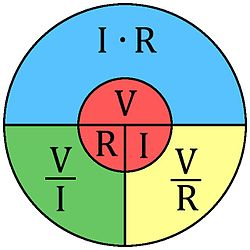
\includegraphics[width=0.5\linewidth]{Images/Ley_de_ohm_-_Organigrama.jpg}
    \end{subfigure}
    \begin{subfigure}{0.42\textwidth}
        \centering
        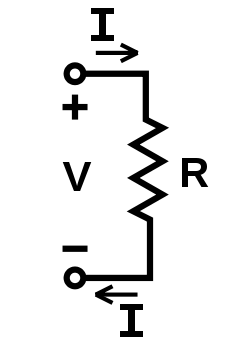
\includegraphics[width=0.5\linewidth]{Images/esquema ohm.png}
    \end{subfigure}
\end{figure}

Por otro lado la resistividad es una magnitud intensiva, depende solo del material y no de su geometría, y se define como la resistencia eléctrica de dicho material. La resistividad y la resistencia del material se relacionan a partir de la siguiente fórmula:

\begin{equation}
    R = \rho \: \frac{L}{S} \Rightarrow \rho = R \: \frac{S}{L}
    \label{Resistividad}
\end{equation}

\newpage

\begin{itemize}
    \item $R$ es la resistencia del material, en el SI se mide en $\Omega$
    \item $S$ es la sección transversal del material
    \item $L$ es la longitud del material
    \item $\rho$ es la resistividad del material, en el SI se mide en $\Omega \cdot m$
\end{itemize}

Valores altos de resistividad indican que el material es un aislante, mientras que valores bajos indican que el material es un buen conductor. Para hacernos una idea, la resistividad de la mayoría de los metales más comunes, como la plata o el oro es del orden de $10^{-8}\: \Omega \cdot m$, mientras que la resistividad de aislantes como la madera o el vidrio puede llegar a valores del orden de $10^{10}\: \Omega \cdot m$.

\section{Materiales y metodología}

La práctica consta de dos partes bien diferenciadas. En primer lugar determinaremos la resistividad del cobre y del aluminio a partir de dos barras metálicas. En la segunda parte el objetivo será determinar la resistencia entre dos contactos de una caja de conexiones realizando medidas con diferentes cables.

\subsection{Determinación de la resistividad de metales}

Los materiales empleados fueron los siguientes:

\begin{itemize}
    \item Dos barras metálicas de los materiales a estudiar, cobre y aluminio
    \item Generador de corriente continua y cables conductores
    \item Amperímetro y voltímetro
    \item Amplificador de señal
\end{itemize}

\newpage

El montaje experimental del circuito es el siguiente:

\begin{figure}[h!]
    \begin{subfigure}{0.5\textwidth}
        \centering
        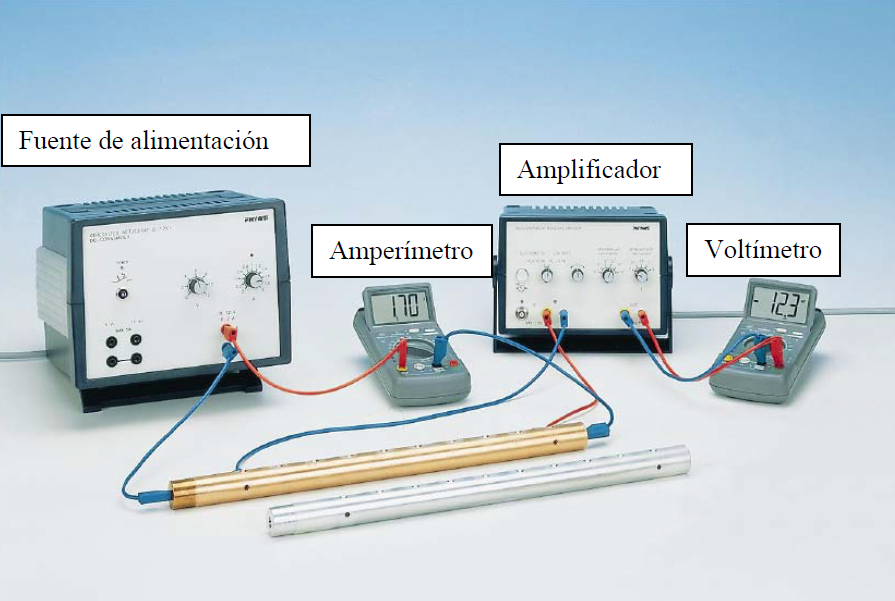
\includegraphics[width=1\linewidth]{Images/montaje experimental.png}
        \subcaption{Material empleado}
    \end{subfigure}
    \begin{subfigure}{0.42\textwidth}
        \centering
        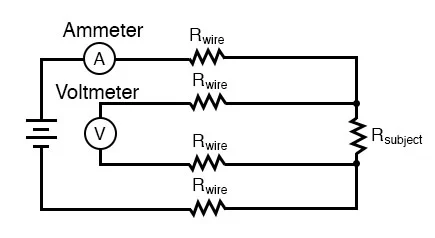
\includegraphics[width=1.5\linewidth]{Images/ohmmeter-example3.png}
        \subcaption{Esquema del circuito}
    \end{subfigure}
    \caption{Montaje experimental}
    \label{Circuito}
\end{figure}



El método utilizado para la medición fue el método de Kelvin o medición a cuatro puntas, como se puede observar en el circuito. En nuestro caso particular el método de la medición a dos puntas, conectando simplemente un óhmetro a cada extremo de la barra, nos proporcionaría un valor lejano al de la resistencia real. Esto se debe a que, pese a ser el método más común, el valor de la resistencia que medimos incluye también la resistencia del cableado, además de la resistencia incógnita. Para resistencias de un valor razonable esta desviación es casi imperceptible, pues la resistencia de los cables es muy baja. No obstante, estamos trabajando con metales conductores que cuentan con una resistencia muy baja, por lo que la interferencia del cableado provocaría que las medidas estuvieran muy lejos de las reales. La ventaja del método de Kelvin es que nos permite medir la resistencia incógnita de forma indirecta a partir de la ley de Ohm, debido a que la intensidad de corriente permanece constante en todo el circuito lo único que necesitamos medir es la caída de potencial entre los contactos de nuestra barra metálica. Además de esto, hay que señalar que, puesto que la resistencia de los voltímetros es muy alta, prácticamente no circula corriente por el circuito interno por lo que la caída de potencial que medimos se puede atribuír totalmente a la barra metálica.

\par Como bien hemos señalado antes, la medida de la resistencia se realizará de forma indirecta a partir de la ley de Ohm. Mediremos 20 pares de valores de intensidad y voltaje distribuidos de forma uniforme entre los $0 \; A$ y los $4 \; A$ que puede suministrar la fuente de alimentación como máximo, separando cada medida por $0,2 \; A$. Para medir el voltaje necesitaremos un amplificador de señal, puesto que la caída de potencial entre los contactos es muy baja. En nuestro caso (Para ambas barras metálicas) el factor de amplificación será de $10^2$, por lo que el resultado medido deberá ser dividido por $100$. Una vez tengamos nuestros $20$ valores de intensidad y voltaje realizaremos un ajuste por mínimos cuadrados para calcular la resistencia.

\par Un último detalle a destacar en la medida de las caídas de potencial (Voltaje) es el efecto del voltaje residual. Como estamos trabajando con un factor de amplificación $100$ la magnitud de la electricidad residual del circuito toma cierta importancia, esto se traduce en que a intensidad cero exista un pequeño voltaje residual que modifica el cero del voltaje. Este efecto debe tenerse en cuenta a la hora de medir la caída de potencial de la barra metálica y puede corregirse de la siguiente forma:

\begin{figure}[h!]
    \centering
    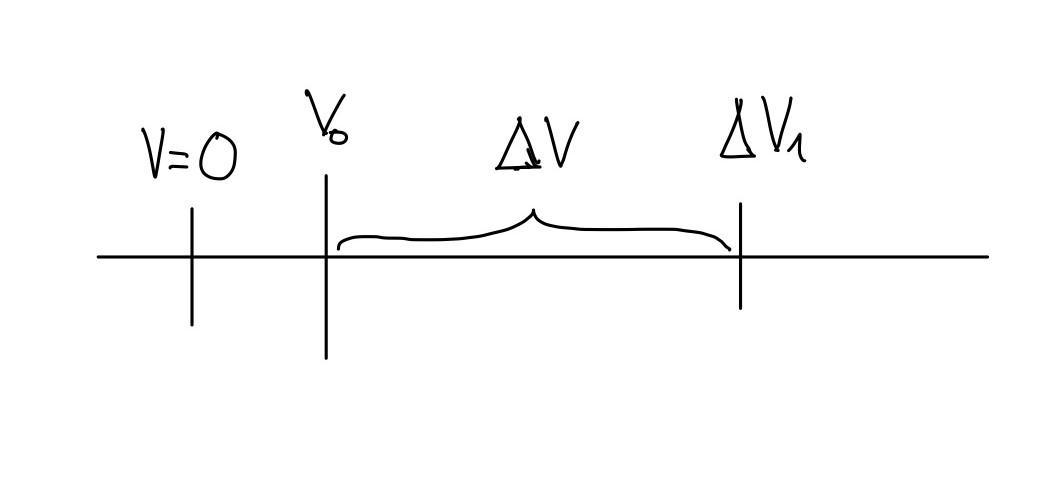
\includegraphics[width=0.65\linewidth]{Images/voltaje residual-4 (002).jpg}
    \caption{Esquema del efecto del voltaje residual}
\end{figure}

\begin{equation}
    \Delta V = \Delta V_{1} - V_{0}
    \label{Voltaje residual}
\end{equation}

Donde $\Delta V$ es la caída de potencial real, $\Delta V_{1}$ es la caída medida y $V_{o}$ es el voltaje residual.

Por tanto, la incertidumbre de la caída de potencial tiene la siguiente expresión:

\begin{equation}
    s(\Delta V) = \sqrt{\left (\frac{\partial \Delta V_{1}}{\partial \Delta V}\right )^2s^2(\Delta V_{1}) + \left (\frac{\partial V_{0}}{\partial \Delta V}\right )^2s^2(V_{o})} = \sqrt{s^2(\Delta V_{1}) + s^2(V_{0})}
    \label{Inc Voltaje residual}
\end{equation}

Como la incertidumbre de todos los voltajes medidos es la misma, podemos expresar la incertidumbre de la caída de potencial real de la siguiente forma:

\begin{equation}
    s(\Delta V) = \sqrt{2}\cdot s(\Delta V_{1})
    \label{Inc voltaje}
\end{equation}

\newpage

\par Una vez conocido el valor de la resistencia de la barra metálica podemos determinar su resistividad a partir de la Ec.\ref{Resistividad}, midiendo la distancia entre contactos y la sección transversal. Además de eso, calcularemos la incertidumbre de la resistividad a partir de propagación de incertidumbres de la siguiente forma:

\begin{align}
    s(\rho) &= \sqrt{\left (\frac{\partial \rho}{\partial R}\right )^2s^2(R)  +  \left (\frac{\partial \rho}{\partial L}\right )^2s^2(L)  +  \left (\frac{\partial \rho}{\partial S}\right )^2s^2(S)} \nonumber \\
    s(\rho) &= \sqrt{\left (\frac{S}{L}\right )^2s^2(R)  +  \left (\frac{-RS}{L^2}\right )^2s^2(L)  +  \left (\frac{R}{L}\right )^2s^2(S)}
    \label{Inc resistividad}
\end{align}

El valor de la sección transversal se obtiene midiendo el radio y calculando el área del círculo por lo que su incertidumbre es la siguiente:

\begin{align}
    \begin{split}
    S &= \pi r^2 \\
    s(S) = \sqrt{\left (\frac{\partial S}{\partial r}\right )^2s^2(S)} &= 2\pi r s(r)
    \end{split}
    \label{Inc sección}
\end{align}

Las incertidumbres del diámetro de la barra metálica y de la distancia entre contactos vienen dadas por el aparato de medida, la regla, que contaba con una incertidumbre de $0,5 \; mm = 0,0005 \; m$. Por tanto, la incertidumbre del radio será la mitad de la del diámetro.

\begin{align}
    \begin{split}
        s(r) &=\frac{s(d)}{2}= 0,00025 m  \\
        s(L) &= 0,0005 m
    \end{split}
\end{align}

Por último, cabe destacar que ciertos valores de voltaje medidos son el valor medio entre los límites de oscilación del voltímetro, pues la amplifiación provocaba cierta oscilación en el voltaje. No obstante, para realizar el tratamiento de datos hemos considerado tomar todos los valores con una incertidumbre constante, el doble de la dada por el voltímetro. La justificación para hacer esto es que las oscilaciones no provocaban cambios excesivos en el valor y este terminaba por estabilizarse entorno a un voltaje determinado. Por tanto, todos los ajustes por mínimos cuadrados realizados fueron regresiones lineales simples sin término independiente, que se explican detalladamente en la parte de mecánica.

\newpage

\subsection{Determinación de la resistencia entre contactos de la caja de conexiones}

Los materiales empleados fueron los siguientes:

\begin{itemize}
    \item Caja de conexiones
    \item Generador de corriente continua y cableado
    \item Tres cables conductores de diferentes longitudes: 2000 mm, 600 mm, 100 mm
    \item Amperímetro y voltímetro
\end{itemize}

El esquema del montaje experimental es el siguiente:

\begin{figure}[h!]
    \centering
    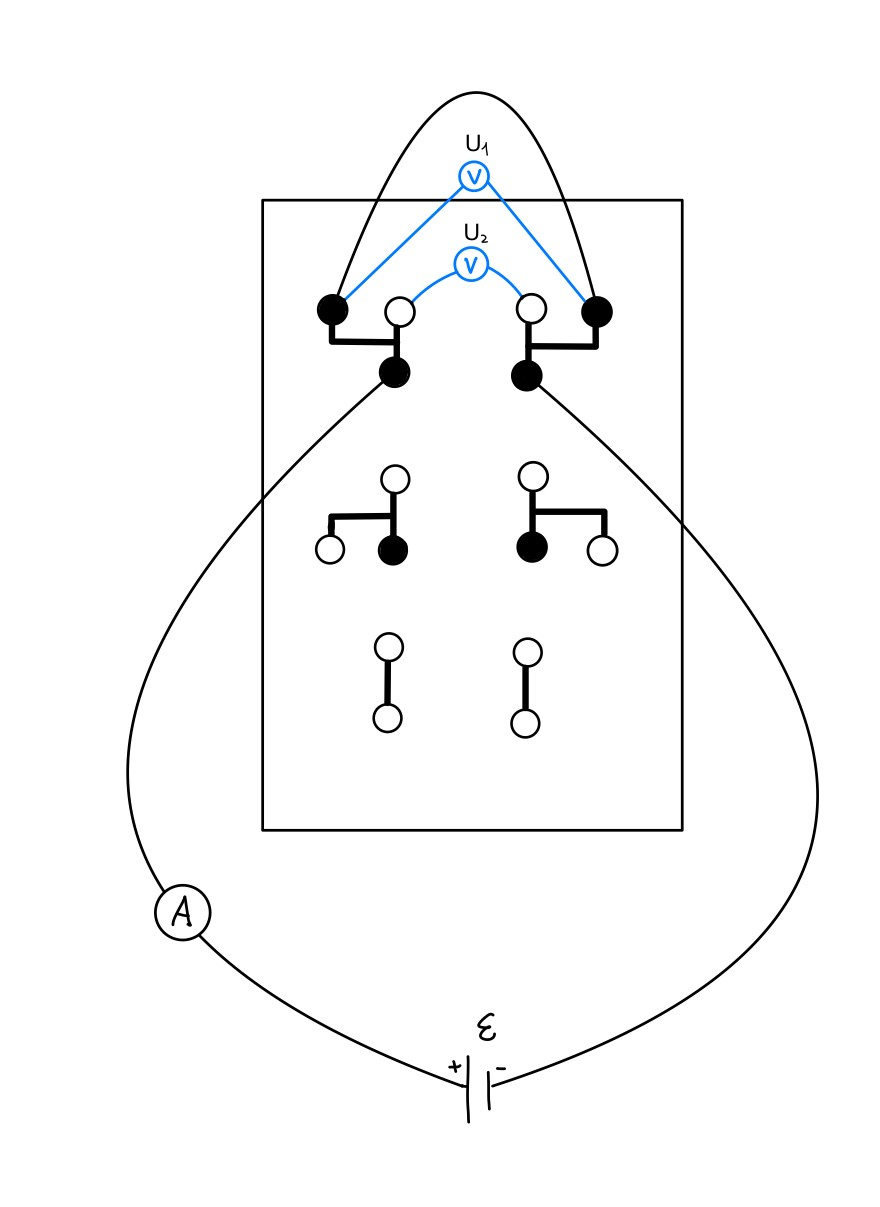
\includegraphics[width=0.65\linewidth]{Images/esquema caja conexiones.jpeg}
    \caption{Esquema del circuito experimental}
    \label{Caja de conexiones}
\end{figure}

En el esquema podemos observar dos posibles configuraciones del voltímetro, $U_{1}$ y $U_{2}$. En la configuración $U_{1}$ conectamos el voltímetro directamente al cable, por lo que la caída de potencial medida se debe únicamente a los diferentes cables conductores. Por otra parte, en la configuración $U_{2}$ conectamos el voltímetro a los contactos libres, por lo que la caída de potencial medida se debe al cableado y a los contactos entre los conductores.

\par Las medidas se realizarán de forma idéntica a las realizadas en el apartado anterior, mediremos los valores de voltaje provocados por diferentes intensidades distribuidas uniformemente en el rango de $0$ a $4 \;A$. A diferencia del apartado anterior, estas medidas fueron tomadas sin amplificación, pues los intentos de trabajar con factores de amplificación de 100 e incluso 10 provocaban oscilaciones muy importantes en la medida. Respecto a las medidas debemos destacar también que en los casos de los cables más largos no fuimos capaces de llegar a los $4 \: A$ de intensidad, pues a partir de valores del orden de $3\; A$ las medidas comenzaban a oscilar y perdían la linealidad.

\par Una vez tengamos los valores de intensidad y voltaje calcularemos la resistencia por un ajuste de mínimos cuadrados en cada caso. La forma de determinar la resistencia entre contactos de la caja de conexiones es la siguiente:

\begin{equation}
    R_{C} = \frac{R_{2}-R_{1}}{2}
    \label{Resistencia contactos}
\end{equation}

La resistencia entre contactos se calcula restando a la resitencia total la resistencia del cable y dividiendo entre dos, para calcular la resistencia solo entre los contactos de un lado. La incertidumbre asociada es la siguiente:

\begin{equation}
    s(R_{C}) = \sqrt{\left (\frac{\partial R_{C}}{\partial R_{2}}\right )^2s^2(R_{2})  +  \left (\frac{\partial R_{C}}{\partial R_{1}}\right )^2s^2(R_{1})} = \frac{1}{2}\sqrt{s^2(R_{2})  +  s^2(R_{1})}
    \label{Inc Resistencia caja}
\end{equation}

Obtendremos 3 valores de $R_{C}$ para cada uno de los tres cables (100 mm, 600 mm y 2000 mm) con los cuales podremos determinar el valor de la resistencia entre contactos calculando su media aritmética.

\newpage

\section{Análisis de datos}

\subsection{Resistividad del cobre}

Como se ha detallado en la metodología, tomamos 20 valores de intensidad y voltaje, que serán representados en una tabla a continuación.

\par La incertidumbre de la intensidad viene dada por la fuente de alimentación:

\begin{equation}
    s(I) = 0,01 \; A
\end{equation}

La incertidumbre del voltaje medido, como hemos explicado antes, debe tener en cuenta el factor de amplificación y además la escala del voltímetro, que para estas medidas estaba en $mV$. Por tanto, teniendo en cuenta que trabajamos con un factor de amplificación 100 debemos dividir todos los resultados entre $10^5$ para obtener los valores en unidades del SI. La incertidumbre del voltímetro era de $0,1 \; mV$, por tanto la incertidumbre de nuestras medidas fue de:

\begin{equation}
    s(\Delta V_{1}) = 2 \cdot 10^{-6}\; V
\end{equation}

Debemos tener en cuenta el valor del voltaje residual, que afectará a nuestra incertidumbre, como hemos mencionado anteriormente, por lo que el valor final de la incertidumbre de las caídas de potencial es:

\begin{equation}
    s(\Delta V) = \sqrt{2}\cdot s(\Delta V_{1}) = 2,8 \cdot 10^{-6} \; V
\end{equation}

\bigskip

\begin{table}[h!]
    \centering
    \begin{tabular}{|c|c|c|c|}
        \hline Intensidad($A$) & Voltaje($mV$) & Intensidad($A$) & Voltaje($mV$) \\
        \hline
        $0,2$ & $0,005$ & $2,2$ & $0,028$\\
        \hline
        $0,4$ & $0,007$ & $2,4$ & $0,030$  \\
        \hline
        $0,6$ & $0,009$ & $2,6$ & $0,032$  \\
        \hline
        $0,8$ & $0,013$ & $2,8$ & $0,034$  \\
        \hline
        $1,0$ & $0,015$ & $3,0$ & $0,036$  \\
        \hline
        $1,2$ & $0,016$ & $3,2$ & $0,038$  \\
        \hline
        $1,4$ & $0,018$ & $3,4$ & $0,041$  \\
        \hline
        $1,6$ & $0,020$ & $3,6$ & $0,043$  \\
        \hline
        $1,8$ & $0,023$ & $3,8$ & $0,046$  \\
        \hline
        $2,0$ & $0,026$ & $4,0$ & $0,048$  \\
        \hline
    \end{tabular}
    \caption{Medidas de la barra de cobre}
\end{table}

Los datos medidos están expresados en $mV$ y quitando ya el efecto de la amplificación y del voltaje residual (Ec.\ref{Voltaje residual}, donde el valor del cero resultó ser de $14,8 \; mV$), para trabajar con las caídas de potencial reales.

\par A partir de estos datos vamos a hacer una regresión lineal simple sin término independiente por el método de los mínimos cuadrados para aproximar nuestros puntos experimentales a una recta del tipo $y=bx$ usando las Ec.8, Ec.9, Ec.10 y Ec.11. La variable dependiente ($y$) será la intensidad y la variable dependiente ($x$) será el voltaje. Los valores obtenidos fueron:

\begin{equation}
    \begin{gathered}
        b = 1.226 \cdot 10^{-5}\; \Omega
        \\
        s(b) = 1.4 \cdot 10^{-7}\; \Omega
        \\
        r = 0.998
        \\
        s = 1.5 \cdot 10^{-6}
    \end{gathered}
\end{equation}

Por tanto la recta a la que aproximamos nuestros puntos tiene la siguiente ecuación:

\begin{equation}
    y = 1,226 \cdot 10^{-5}x
\end{equation}

Donde la pendiente de la recta, haciendo una similitud de la ley de Ohm ($V=IR$), resulta ser la resistencia de la barra de cobre $(1,226 \cdot 10^{-5}\;  \Omega)$.

\begin{figure}[h!]
    \centering
    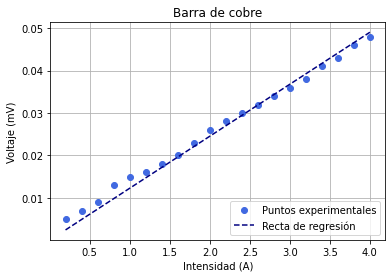
\includegraphics[width=0.85\linewidth]{Images/plotCobre.png}
    \caption{Datos experimentales y recta de regresión de la barra de cobre}
\end{figure}

\newpage

\par A partir del valor de la resistencia de la barra y de los datos de su geometría podemos calcular el valor de la resistividad del cobre a partir de la Ec.\ref{Resistividad}.

\par Los valores medidos de la distancia entre contactos y radio son:

\begin{align}
    \begin{split}
        r &= 0,0125\; m\\
        L &= 0,325\; m
    \end{split}
\end{align}

Entonces su sección transversal es:

\begin{equation}
    S = \pi r^2 = 4,9 \cdot 10^{-4}\; m^2
\end{equation}

\begin{equation}
    \rho_{Cu} = R \: \frac{S}{L} = 1.851 \cdot 10^{-8} \; \Omega \cdot m
\end{equation}

Las incertidumbres asociadas, calculadas a partir de las Ec.\ref{Inc resistividad} y Ec.\ref{Inc sección}, son:

\begin{equation}
    \begin{gathered}
        s(S) = 2\pi r s(r) = 2,0 \cdot 10^{-5} \; m^2
        \\
        s(\rho_{Cu}) = 7.7 \cdot 10^{-10} \; \Omega \cdot m
    \end{gathered}
\end{equation}

Por tanto, el valor final de la resistividad del cobre es de:

\begin{equation}
    \rho_{Cu} = 1.851 \cdot 10^{-8} \pm 7.7 \cdot 10^{-10} \; \Omega \cdot m
\end{equation}

El valor real de la resistividad del cobre es de $1,678 \cdot 10^{-8} \Omega \cdot m$, que aunque no entra en el rango de incertidumbre se encuentra muy cerca del valor experimental.

\subsection{Resistividad del aluminio}

El procedimiento para determinar la resistividad del aluminio es exactamente idéntico, tomaremos los 20 valores de voltaje e intensidad y después realizaremos un ajuste por el método de los mínimos cuadrados para calcular la resistencia de la barra de aluminio valiéndonos de la ley de Ohm. Como el factor de amplificación es el mismo y los aparatos de medida trabajan con la misma escala las incertidumbres en los valores de las caídas de potencial e intensidades no cambian.

\begin{equation}
    \begin{gathered}
    s(I) = 0,01 \; A\\    
    s(\Delta V) = 2,8 \cdot 10^{-6} \; V
    \end{gathered}
\end{equation}

\newpage

Los valores medidos fueron los siguientes (Expresados sin amplificación):

\begin{table}[h!]
    \centering
    \begin{tabular}{|c|c|c|c|}
        \hline
        Intensidad (A) & Voltaje (mV) & Intensidad (A) & Voltaje (mV) \\
        \hline
        $0,2$ & $0,002$ & $2,2$ & $0,039$ \\
        \hline
        $0,4$ & $0,005$ & $2,4$ & $0,041$ \\
        \hline
        $0,6$ & $0,010$ & $2,6$ & $0,045$ \\
        \hline
        $0,8$ & $0,015$ & $2,8$ & $0,048$ \\
        \hline
        $1,0$ & $0,017$ & $3,0$ & $0,051$ \\
        \hline
        $1,2$ & $0,020$ & $3,2$ & $0,054$ \\
        \hline
        $1,4$ & $0,023$ & $3,4$ & $0,058$ \\
        \hline
        $1,6$ & $0,028$ & $3,6$ & $0,061$ \\
        \hline
        $1,8$ & $0,031$ & $3,8$ & $0,065$ \\
        \hline
        $2,0$ & $0,035$ & $4,0$ & $0,069$ \\
        \hline
    \end{tabular}
    \caption{Datos experimentales de la barra de aluminio}
\end{table}

Los datos serán ajustados a una recta del tipo $y=bx$ por un ajuste de mínimos cuadrados igual que en apartado anterior, donde $b$ representa la resistencia. Los valores obtenidos fueron:

\begin{equation}
    \begin{gathered}
        b = R = 1.7120 \cdot 10^{-5} \; \Omega \\
        s(b) = s(R) = 7,7 \cdot 10^{-8} \; \Omega\\
        r = 0,9998 \\
        s = 8,3\cdot 10^{-7}
    \end{gathered}
\end{equation}

Por tanto, la recta de regresión a la que vamos a aproximar nuestros puntos experimentales es la siguiente:

\begin{equation}
    y = 1.226 \cdot 10^{-5}x
\end{equation}

\begin{figure}[h!]
    \centering
    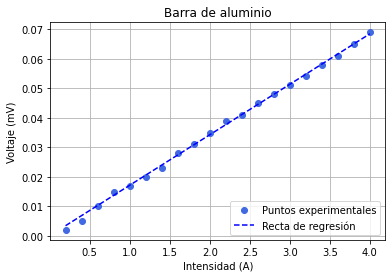
\includegraphics[width=0.85\linewidth]{Images/plotAluminio.png}
    \caption{Datos experimentales y recta de regresión de la barra de aluminio}
\end{figure}

\newpage

Las dimensiones de la barra son las misma, tanto en radio como en distancia entre contactos, por lo que las incertidumbres se mantienen:

\begin{equation}
    \begin{gathered}
        s(S) = 2,0\cdot 10^{-5} \; m^2 \\
        s(L) = 0,0005m
    \end{gathered}
\end{equation}

El valor de la resistencia de la barra es:

\begin{equation}
    R = 1.226 \cdot 10^{-5} \pm 1.4 \cdot 10^{-7} \; \Omega
\end{equation}

Aplicando la Ec.\ref{Resistividad} y la Ec.\ref{Inc resistividad} el valor de la resistividad del aluminio y su incertidumbre es de:

\begin{equation}
    \rho_{Al} = 2.58 \cdot 10^{-8} \pm
    1.0\cdot 10^{-9} \; \Omega \cdot m
\end{equation}

El valor real de la resistividad del aluminio es de $2,650 \cdot 10^{-8} \; \Omega \cdot m$, por lo que nuestro resultado se ajusta en gran medida a la realidad.

\newpage

\subsection{Determinación de la resistencia entre contactos de la caja de conexiones}

Como hemos mencionado en la metodología para la determinación de la resistencia entre contactos vamos a medir la resistencia por dos caminos ($U_{1}$ y $U_{2}$), de forma que a partir de la Ec.\ref{Resistencia contactos} podremos calcular la resistencia entre contactos. Las medidas se realizarán igual que en las barras metálicas, 20 pares de valores (En algunos casos menos por problemas técnicos) de intensidad y voltaje para los caminos $U_{1}$ y $U_{2}$ con tres cables de longitud diferente. A partir de ahí obtendremos tres valores de la resistencia entre contactos que deberemos comparar.

\subsubsection{Cable de 100 mm}

Los valores de intensidad y voltaje medidos para el segmento $U_{1}$, formado solo por el cable, son los siguientes:

\begin{table}[h!]
\centering
    \begin{tabular}{|c|c|c|c|}
        \hline
        Intensidad (A) & Voltaje (mV) & Intensidad (A) & Voltaje (mV) \\ \hline
        $0,2$ & $1,61$ & $2,2$ & $20,0$ \\ \hline
        $0,4$ & $3,5$ & $2,4$ & $21,5$ \\ \hline
        $0,6$ & $5,3$ & $2,6$ & $23,2$ \\ \hline
        $0,8$ & $7,1$ & $2,8$ & $25,6$ \\ \hline
        $1,0$ & $8,9$ & $3,0$ & $27,2$ \\ \hline
        $1,2$ & $10,9$ & $3,2$ & $29,2$ \\ \hline
        $1,4$ & $13,0$ & $3,4$ & $30,7$ \\ \hline
        $1,6$ & $14,6$ & $3,6$ & $32,6$ \\ \hline
        $1,8$ & $16,5$ & $3,8$ & $34,9$ \\ \hline
        $2,0$ & $18,1$ & $4,0$ & $35,7$ \\ \hline
    \end{tabular}
    \caption{Datos experimentales del cable de 100 mm}
\end{table}

A partir de estos datos vamos a realizar un ajuste por el método de los mínimos cuadrados donde ajustaremos nuestros datos experimentales a una recta del tipo $y=bx$. Haciendo una similitud con la ley de Ohm $(V=IR)$, la pendiente de la recta será la resistencia del cable. Los parámetros obtenidos fueron los siguientes:

\begin{equation}
    \begin{gathered}
        b =R_{1}= 0.009058 \; \Omega 
        \\
        s(b) = s(R_{1})= 2.2 \cdot 10^{-5} \; \Omega
        \\
        r = 0.99994
        \\
        s = 0.00024
    \end{gathered}
\end{equation}

Por tanto la recta a la que aproximaremos nuestros puntos es:

\begin{equation}
    y = 0,009058x
\end{equation}

Los valores obtenidos para el segmento $U_{2}$, formado por el cable y la caja de conexiones, son los siguientes:

\begin{table}[h!]
    \centering
    \begin{tabular}{|c|c|c|c|}
        \hline
        Intensidad (A) & Voltaje (mV) & Intensidad (A) & Voltaje (mV) \\
        \hline
        $0,2$ & $4,2$ & $2,2$ & $47,6$ \\
        \hline
        $0,4$ & $8,6$ & $2,4$ & $51,9$ \\
        \hline
        $0,6$ & $12,9$ & $2,6$ & $56,2$ \\ 
        \hline
        $0,8$ & $17,2$ & $2,8$ & $60,5$ \\
        \hline
        $1,0$ & $21,5$ & $3,0$ & $64,4$ \\
        \hline
        $1,2$ & $25,9$ & $3,2$ & $68,7$ \\
        \hline
        $1,4$ & $30,1$ & $3,4$ & $73,0$ \\ 
        \hline
        $1,6$ & $34,8$ & $3,6$ & $77,3$ \\
        \hline
        $1,8$ & $39,0$ & $3,8$ & $81,5$ \\
        \hline
        $2,0$ & $43,3$ & $4,0$ & $85,8$ \\ 
        \hline
    \end{tabular}
    \caption{Datos experimentales del cable de 100 mm y la caja de conexiones}
\end{table}

A partir de estos datos vamos a realizar un ajuste por el método de los mínimos cuadrados donde ajustaremos nuestros datos experimentales a una recta del tipo $y=bx$. Haciendo una similitud con la ley de Ohm $(V=IR)$, la pendiente de la recta será la resistencia del cable. Los parámetros obtenidos fueron los siguientes:

\begin{equation}
    \begin{gathered}
        b = R_{2} =0,021517 \; \Omega 
        \\
        s(b) =s(R_{2})= 1,9 \cdot 10^{-5} \; \Omega
        \\
        r = 0,999992
        \\
        s = 0,00020
    \end{gathered}
\end{equation}

Por tanto la recta a la que aproximaremos nuestros puntos es:

\begin{equation}
    y = 0,021517x
\end{equation}

Cabe destacar que en los valores de caída de potencial reflejados en las tablas ya hemos tenido en cuenta el valor del voltaje residual, que situaba al cero en un valor de $0,4 \; mV$. Para corregir este efecto aplicamos la Ec.\ref{Voltaje residual} y restamos el valor del cero residual a todos los valores medidos. Esta correción afecta a la incertidumbre y tendremos que aplicar la Ec.\ref{Inc voltaje}.

\newpage

\par A diferencia de los apartados anteriores, al no estar trabajando con el amplificador, los valores medidos en el voltímetro no oscilaban, por lo que hemos considerado la incertidumbre del propio voltímetro $(0,1 \; mV=10 \cdot 10^{-4} \; V)$ como la incertidumbre de las caídas de potencial medidas.

\begin{equation}
    s(\Delta V) = \sqrt{2}\cdot 10^{-4} \; V
\end{equation}

La incertidumbre de la intensidades la misma, pues depende solo de la fuente de alimentación:

\begin{equation}
    s(I) = 0,01 \; A
\end{equation}

Finalmente, en la siguiente figura podremos ver la representación gráfica de nuestros ajustes:

\begin{figure}[h!]
    \centering
    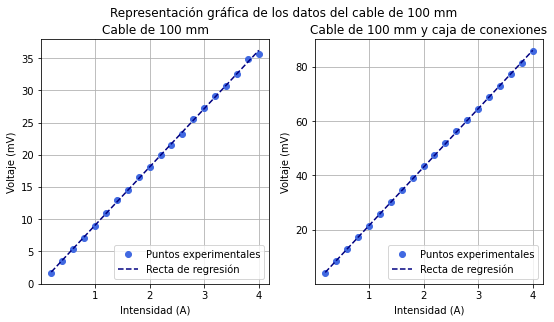
\includegraphics[width=0.9\linewidth]{Images/plotCable1.png}
    \caption{Representación gráfica de los datos experimentales del cable de 100 mm}
\end{figure}

A partir de los ajustes podemos calcular la resistencia entre contactos de la caja de conexiones y su incertidumbre usando la Ec.\ref{Resistencia contactos} y la Ec.\ref{Inc Resistencia caja}:

\begin{equation}
    \begin{gathered}
        R_{C1} = 0.006230 \; \Omega\\
        s(R_{C1}) = 1.5 \cdot 10^{-5} \Omega
    \end{gathered}
\end{equation}

\newpage

\subsubsection{Cable de 600 mm}

El procedimiento será el mismo que para el cable de 100 mm, en primer lugar tomaremos 20 valores de intensidad y voltaje. A diferencia del apartado anterior no había voltaje residual a la hora de realizar las medidas por lo que la incertidumbre del voltaje será menor y será la del propio voltímetro, pues tampoco había oscilaciones en el valor medido. La incertidumbre de la intensidad es la misma.

\begin{equation}
    \begin{gathered}
        s(\Delta V) = 10^{-4} \; V \\
        s(I) = 0,01\; A
    \end{gathered}
\end{equation}

Los valores medidos para el segmento $U_{1}$, formado solo por el cable, fueron los siguientes:

\begin{table}[h!]
    \centering
    \begin{tabular}{|c|c|c|c|}
        \hline
        Intensidad (A) & Voltaje (mV) & Intensidad (A) & Voltaje (mV) \\
        \hline
        $0,2$ & $4,2$ & $2,2$ & $47,4$ \\
        \hline
        $0,4$ & $8,5$ & $2,4$ & $51,7$ \\
        \hline
        $0,6$ & $12,8$ & $2,6$ & $56,1$ \\
        \hline
        $0,8$ & $17,1$ & $2,8$ & $60,4$ \\
        \hline
        $1,0$ & $21,4$ & $3,0$ & $64,8$ \\
        \hline
        $1,2$ & $25,8$ & $3,2$ & $69,2$ \\
        \hline
        $1,4$ & $30,1$ & $3,4$ & $73,6$ \\
        \hline
        $1,6$ & $34,4$ & $3,6$ & $77,9$ \\
        \hline
        $1,8$ & $38,7$ & $3,8$ & $82,4$ \\
        \hline
        $2,0$ & $43,0$ & $4,0$ & $86,8$ \\
        \hline
    \end{tabular}
    \caption{Datos experimentales del cable de 600 mm (Segemto $U_{1}$)}
\end{table}

A partir de estos datos vamos a realizar un ajuste por el método de los mínimos cuadrados donde ajustaremos nuestros datos experimentales a una recta del tipo $y = bx$. Haciendo una similitud con la ley de Ohm (V = IR), la pendiente de la recta será la resistencia del cable. Los parámetros obtenidos fueron los siguientes:

\begin{equation}
    \begin{gathered}
        b = R_{1}=  0.021611 \; \Omega \\
        s(b)= s(R_{1}) = 1.7 \cdot 10^{-5} \; \Omega \\
        r =  0.999994 \\
        s =  0.00018
    \end{gathered}
\end{equation}

Por tanto la recta a la que aproximamos nuestros datos es:

\begin{equation}
    y = 0.021611x
\end{equation}

Para el segmento $U_{2}$, formado por el cable de 600 mm y la caja de conexiones, hay que señalar que , como mencionamos en la metodología, a partir de ciertos valores de intensidad los voltajes medidos comenzaron a oscilar y perder la linealidad. Por este motivo nuestras medidas solo llegan a los $3,4$ A de intensidad. Los valores obtenidos fueron los siguientes:

\begin{table}[h!]
    \centering
    \begin{tabular}{|c|c|c|c|}
        \hline
        Intensidad (A) & Voltaje (mV) & Intensidad (A) & Voltaje (mV) \\
        \hline
        $0,2$ & $11,4$ & $2,0$ & $113,3$ \\
        \hline
        $0,4$ & $22,8$ & $2,2$ & $124,5$ \\
        \hline
        $0,6$ & $34,0$ & $2,4$ & $135,6$ \\
        \hline
        $0,8$ & $45,4$ & $2,6$ & $146,7$ \\
        \hline
        $1,0$ & $56,7$ & $2,8$ & $157,9$ \\
        \hline
        $1,2$ & $68,1$ & $3,0$ & $169,1$ \\
        \hline
        $1,4$ & $79,4$ & $3,2$ & $180,3$ \\
        \hline
        $1,6$ & $90,7$ & $3,4$ & $191,4$ \\
        \hline
        $1,8$ & $102$ &  &  \\
        \hline
    \end{tabular}
    \caption{Datos expeerimentales del cable de 600 mm y la caja de conexiones}
\end{table}

A partir de estos datos vamos a realizar un ajuste por el método de los mínimos cuadrados donde ajustaremos nuestros datos experimentales a una recta del tipo $y = bx$. Haciendo una similitud con la ley de Ohm (V = IR), la pendiente de la recta será la resistencia del cable. Los parámetros obtenidos fueron los siguientes:

\begin{equation}
    \begin{gathered}
        b = R_{2} = 0,056455 \; \Omega \\
        s(b) = s(R_{2}) = 3.6 \cdot 10^{-5} \; \Omega \\
        r =  0.999996 \\
        s =  0.00031
    \end{gathered}
\end{equation}

Por tanto la recta a la que aproximamos nuestros datos es:

\begin{equation}
    y = 0,056455x
\end{equation}

En la siguiente figura podemos ver una representación gráfica de nuestros datos experimentales y el resultado del ajuste:

\begin{figure}[h!]
    \centering
    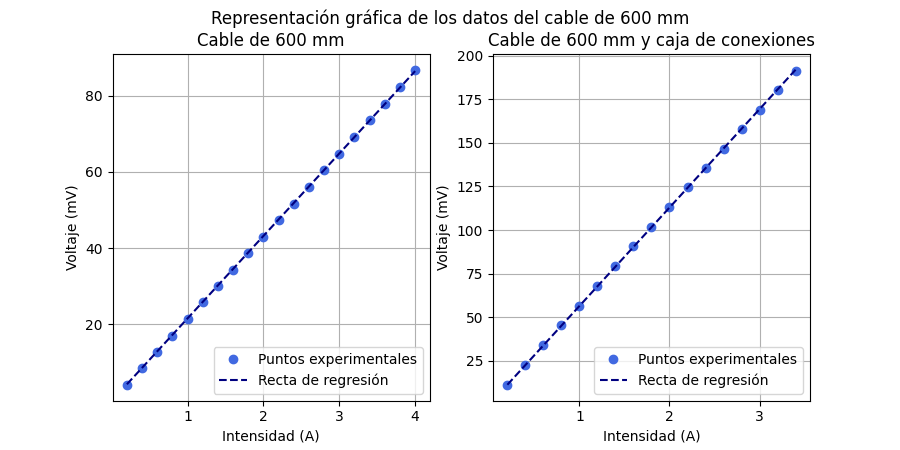
\includegraphics[width=0.95\linewidth]{Images/plotCable2.png}
    \caption{Datos experimentales y rectas de rgresión del cable de 600 mm}
\end{figure}

\newpage

A partir de los ajustes podemos calcular la resistencia entre contactos de la caja de conexiones y su incertidumbre usando la Ec.\ref{Resistencia contactos} y la Ec.\ref{Inc Resistencia caja}:

\begin{equation}
    \begin{gathered}
        R_{C2} = 0.017422 \; \Omega\\
        s(R_{C2}) = 2.6 \cdot 10^{-5}\; \Omega
    \end{gathered}
\end{equation}



\subsubsection{Cable de 2000 mm}

El procedimiento será el mismo que para los otros dos cables, en primer lugar tomaremos 20 valores de intensidad y voltaje. A diferencia del apartado anterior no había voltaje residual a la hora de realizar las medidas por lo que la incertidumbre del voltaje será la del propio voltímetro, pues tampoco había oscilaciones en el valor medido. No obstante los valores de la caída de potencial medidos se pasaban del límite de la escala de 200 mV con la que trabajamos durante toda la práctica, por lo que tuvimos que aumentar la escala y con ello aumenta la incertidumbre. La incertidumbre de la intensidad es la misma.

\begin{equation}
    \begin{gathered}
        s(\Delta V) = 10^{-3} \; V \\
        s(I) = 0,01\; A
    \end{gathered}
\end{equation}

A la hora de realizar las medidas nos encontramos, de la misma forma que en el apartado anterior, que a voltajes altos las medidas comenzaron a oscilar y perdían la linealidad, por lo que realizamos menos medidas. Los valores medidos para el segmento $U_{1}$, formado solo por el cable, fueron los siguientes:

\begin{table}[h!]
    \centering
    \begin{tabular}{|c|c|c|c|}
        \hline
        Intensidad (A) & Voltaje (V) & Intensidad (A) & Voltaje (V) \\ \hline
        $0,2$ & $0,029$ & $1,8$ & $0,302$ \\ \hline
        $0,4$ & $0,061$ & $2,0$ & $0,337$ \\ \hline
        $0,6$ & $0,093$ & $2,2$ & $0,372$ \\ \hline
        $0,8$ & $0,127$ & $2,4$ & $0,407$ \\ \hline
        $1,0$ & $0,163$ & $2,6$ & $0,452$ \\ \hline
        $1,2$ & $0,196$ & $2,8$ & $0,489$ \\ \hline
        $1,4$ & $0,233$ & $3,0$ & $0,525$ \\ \hline
        $1,6$ & $0,267$ & $3,2$ & $0,570$ \\ \hline
    \end{tabular}
    \caption{Datos experimentales del cable de 2000 mm}
\end{table}

A partir de estos datos vamos a realizar un ajuste por el método de los mínimos cuadrados donde ajustaremos nuestros datos experimentales a una recta del tipo $y = bx$. Haciendo una similitud con la ley de Ohm (V = IR), la pendiente de la recta será la resistencia del cable. Los parámetros obtenidos fueron los siguientes:

\begin{equation}
    \begin{gathered}
        b = R_{1} = 0.1720 \; \Omega \\
        s(b) = s(R_{1}) = 0.0012\; \Omega \\
        r =  0.9996 \\
        s =  0.0095
    \end{gathered}
\end{equation}

Por tanto la recta a la que aproximamos nuestros datos es:

\begin{equation}
    y = 0.1720x
\end{equation}

Para el segmento $U_{2}$, formado por el cable de 2000 mm y la caja de conexiones, hay que señalar que , como mencionamos en la metodología, a partir de ciertos valores de intensidad los voltajes medidos comenzaron a oscilar y perder la linealidad. Por este motivo nuestras medidas solo llegan a los $3$ A de intensidad. Los valores obtenidos fueron los siguientes:

\begin{table}[h!]
    \centering
    \begin{tabular}{|c|c|c|c|}
        \hline
        Intensidad (A) & Voltaje (V) & Intensidad (A) & Voltaje (V) \\ \hline
        $0,2$ & $0,064$ & $1,8$ & $0,465$ \\ \hline
        $0,4$ & $0,131$ & $2$ & $0,508$ \\\hline
        $0,6$ & $0,194$ & $2,2$ & $0,532$ \\\hline
        $0,8$ & $0,253$ & $2,4$ & $0,57$ \\\hline
        $1$ & $0,315$ & $2,6$ & $0,602$ \\\hline
        $1,2$ & $0,356$ & $2,8$ & $0,623$ \\\hline
        $1,4$ & $0,4$ & $3$ & $0,664$ \\\hline
        $1,6$ & $0,423$ & & \\
    \hline
    \end{tabular}
    \caption{Datos experimentales del cable de 2000 mm y la caja de conexiones}
\end{table}

\newpage

A partir de estos datos vamos a realizar un ajuste por el método de los mínimos cuadrados donde ajustaremos nuestros datos experimentales a una recta del tipo $y = bx$. Haciendo una similitud con la ley de Ohm (V = IR), la pendiente de la recta será la resistencia del cable. Los parámetros obtenidos fueron los siguientes:

\begin{equation}
    \begin{gathered}
        b = R_{2} = 0.2431 \; \Omega \\
        s(b) = s(R_{2}) = 0.0067\; \Omega \\
        r =    0.994 \\
        s =  0.047
    \end{gathered}
\end{equation}

Por tanto la recta a la que aproximamos nuestros datos es:

\begin{equation}
    y = 0,2431x
\end{equation}

En la siguiente figura podemos ver una representación gráfica de nuestros datos experimentales y el resultado del ajuste:

\begin{figure}[h!]
    \centering
    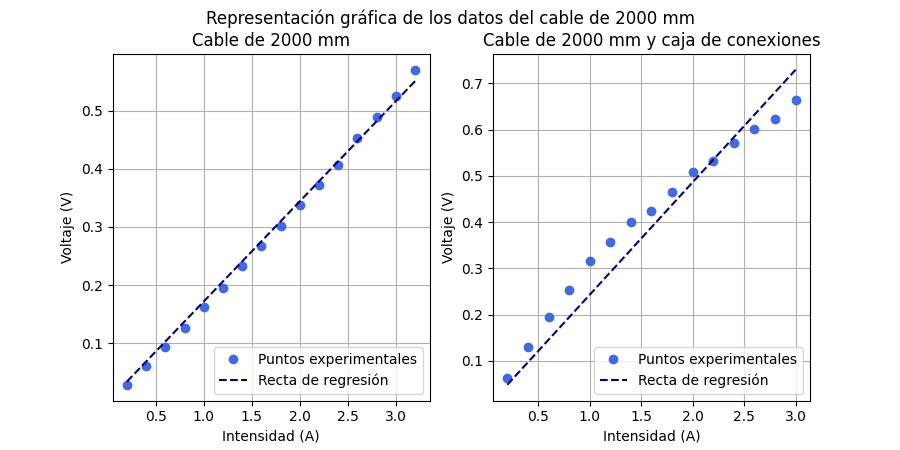
\includegraphics[width=0.95\linewidth]{Images/plotCable3.png}
    \caption{Datos experimentales y rectas de rgresión del cable de 2000 mm}
\end{figure}

\newpage

A partir de los ajustes podemos calcular la resistencia entre contactos de la caja de conexiones y su incertidumbre usando la Ec.\ref{Resistencia contactos} y la Ec.\ref{Inc Resistencia caja}:

\begin{equation}
    \begin{gathered}
        R_{C3} = 0.0355 \; \Omega\\
        s(R_{C3}) = 0.0047\; \Omega
    \end{gathered}
\end{equation}




\newpage

\section{Conclusiones}

Finalmente, vamos a hacer una recapitulación de todos los resultados obtenidos, para poder realizar un análisis global de la práctica. La primera parte de la práctica se centró en determinar la resistividad de dos materiales, el cobre y el aluminio, a partir de la determinación de la resistencia de la barra metálica. Los resultados obtenidos, comparados con los reales obtenidos de \textit{The Handbook of Chemistry and Physics} fueron los siguientes:

\begin{table}[h!]
    \centering
    \begin{tabular}{|c|c|c|}
        \hline
        Material & $\rho_E \pm s(\rho_E) \; (\Omega \cdot m)$ & $\rho \; (\Omega \cdot m)$  \\ \hline
        Cobre  & $1,851 \cdot 10^{-8} \pm 7,7 \cdot 10^{-10}$ & $1.678 \cdot 10^{-8}$ \\ \hline
        Aluminio &$2,58 \cdot 10^{-8} \pm 1,0 \cdot 10^{-9}$ & $2.650\cdot 10^{-8}$\\ \hline
    \end{tabular}
    \caption{Resultados obtenidos para las resistividades}
\end{table}

Como podemos ver, los resultados obtenidos se acercan bastante a los valores reales, las diferencias, pese a que no entran dentro del rango de incertidumbre en el caso del cobre, son muy pequeñas, los valores medidos se corresponden bastante con la realidad. Las pequeñas diferencias las podemos atribuír a los problemas sufridos toda la práctica con los materiales, sobre todo con la fuente de alimentación. Por tanto, podemos concluir que esta primera parte de la práctica fue un éxito.

\par Por otro lado, la segunda parte de la práctica se centró en determinar la resistencia entre contactos de la caja de conexiones. Para ello medimos las diferencias en la resistencia medida solo con el cable y con el cable y la caja de conexiones para tres cables de longitudes diferentes. Los resultados obtenidos de la resistencia entre contactos fueron:

\begin{table}[h!]
    \centering
    \begin{tabular}{|c|c|}
        \hline
        Cable & $R_{C} \pm s(R_C) \; (\Omega)$ \\ \hline
        $100 \; mm$ & $0,006230 \pm 0,000015$\\ \hline
        $600 \; mm$ & $0,017422 \pm 0,000026$\\ \hline
        $2000 \; mm$ & $0,0355 \pm 0,0047$\\ \hline
    \end{tabular}
    \caption{Resultados obtenidos para la resistencia entre contactos}
\end{table}

En esta parte de la práctica los resultados obtenidos difieren bastante más entre sí, llegando las diferencias incluso a un orden de magnitud entre la medida con el primer cable y las otras dos. No obstante, en esta parte de la práctica era hasta cierto punto esperable obtener esas diferencias, sobre todo al trabajar con los cables más largos. Este error sistemático se puede explicar porque las resistencias de los cables con los que trabajamos son notablemente mayores que la resistencia entre contactos de la caja de conexiones, por lo que cualquier falta de precisión en la medida de la resistencia de los cables puede provocar variaciones muy grandes en el valor obtenido de la resistencia entre contactos.

\par Además de eso, otra posible causa para esas diferencias es el mal funcionamiento del material empleado. Como ya hemos explicado anteriormente, al trabajar con intensidades altas en los cables más largos (Por encima de 3 A) los valores de voltaje medidos perdían la linealidad y la fiabilidad. Debido a esto tomamos menos medidas que en el primer cable y las medidas que tomamos probablemente no se ajustarán del todo a los valores reales.

\par Finalmente, pese a todo podemos considerar que hemos alcanzado los objetivos propuestos en la práctica. Conseguimos determinar la resistividad del cobre y del aluminio, obteniendo valores fiables, y conseguimos determinar la resistencia entre contactos de la caja de conexiones, teniendo en cuenta el error sistemático comentado. Además de eso adquirimos una gran experiencia en el manejo de aparatos eléctricos, como la fuente de alimentación, los multímetros y el amplificador.

\section{Bibliografía}

\begin{itemize}
    \item Guión y vídeo explicativo de la práctica de pequeñas resistencias. Campus virtual USC, técnicas experimentales I.
    \item \item Teoría de análisis de incertidumbres. Campus virtual USC, técnicas experimentales I.
    \item \textit{The Handbook of Chemistry and Physics}, 2005
    \item \url{https://es.wikipedia.org/wiki/Ley_de_Ohm}
\end{itemize}

\end{document}